%% Wave Motion submission draft, built on the Elsevier elsarticle template
%% (same class, bibliography style and format as ../wavemotion-paper).
%% Build: ./build.sh     Tables: python make_tables.py (written from the run data)
%% TODO before submission: confirm the author list and affiliations, complete the
%% CRediT statement and funding, and read every reference against the final text.

\documentclass[preprint,12pt]{elsarticle}

\usepackage{amsmath,amssymb,bm}
\usepackage{booktabs}
\usepackage{float}
\usepackage{graphicx}
\usepackage{placeins}

\journal{Wave Motion}

\graphicspath{{./figures/}}

\newcommand{\mbf}[1]{\mathbf{#1}}
\newcommand{\be}{\begin{equation}}
\newcommand{\ee}{\end{equation}}
\newcommand{\bsigma}{\boldsymbol{\sigma}}
\newcommand{\er}{\mbf{e}_r}
\newcommand{\et}{\mbf{e}_\theta}
\newcommand{\qedbox}{\hfill$\square$}

\newtheorem{theorem}{Theorem}
\newtheorem{proposition}{Proposition}
\newtheorem{remark}{Remark}
\newproof{pf}{Proof}

\begin{document}

\begin{frontmatter}
\title{Regularised transformation-elastic cloaking of a circular cavity embedded in an
elastic medium: formulation and finite-element validation for bulk waves}

%% TODO: author list carried over from the group's Wave Motion draft; confirm.
\author[1,2]{David Aznaurov}
\author[1]{David Piliposyan}
\author[1]{Danila Rukhovich}
\author[3]{S\'ebastien Guenneau}

\affiliation[1]{organization={M:3L Lab, Institute of Mechanics, 24B Baghramyan Ave., 0019 Yerevan},
                country={Armenia}}
\affiliation[2]{organization={Biutopic, 18 Rue Paul Ramadier, 44201 Nantes}, country={France}}
\affiliation[3]{organization={The Blackett Laboratory, Department of Physics, UMI 2004 Abraham de Moivre-CNRS, Imperial College London},
                addressline={London SW7 2AZ},
                country={United Kingdom}}

\begin{abstract}
We study the continuous transformation-elastic cloak for a traction-free circular cavity fully
embedded in an isotropic elastic medium and excited by a localised harmonic force that radiates
both pressure and shear waves. The singular radial map is replaced by a map from
$\varepsilon\le R\le b$ onto $a\le r\le b$, and the full Brun--Guenneau--Movchan tensor is kept,
without minor symmetry. We prove that the regularised cloak reproduces outside $r=b$ exactly the
field of a traction-free hole of radius $\varepsilon$ in the background, which provides an exact
reference for separating regularisation error from implementation and discretisation error. The
problem is solved with quadratic finite elements and a perfectly matched layer. The numerical
model is verified against a closed-form Green tensor, a superposition identity and a mirror symmetry,
all proved here. At $\varepsilon/a=0.01$ and $b=\lambda_S$, the normalised exterior error in total
displacement magnitude is $6.7\times10^{-5}$, against $0.158$ for the uncloaked cavity. The error
scales as $\varepsilon^2$. Across six combinations of source position and force direction and for
$0.1\le b/\lambda_S\le 2.5$, it stays between $2\times10^{-6}$ and $3\times10^{-4}$, whereas the uncloaked
cavity reaches $0.2$. These results establish a validated reference for
later approximations of the cloak by realisable materials.
\end{abstract}

\begin{keyword}
elastic cloaking \sep transformation elasticity \sep bulk waves \sep near-cloak \sep
perfectly matched layer \sep finite elements
\end{keyword}

\end{frontmatter}

%% =============================================================
\section{Introduction}\label{sec:intro}
%% =============================================================

Transformation methods design a material distribution from a coordinate map, so that waves pass
around a region as if it were absent~\citep{pendry2006}. In elasticity, the Navier equations are
not form invariant under a general map~\citep{milton2006}, and the choice of the relation between the
displacements in the virtual and physical domains determines the required
medium~\citep{norris2011}. With the gauge $\mbf{U}(\mbf{X})=\mbf{u}(\mbf{x})$, the transformed
stiffness keeps its major symmetry but loses its minor symmetries while the density remains
scalar~\citep{brun2009,norris2011}. This is a Cosserat-type medium, which ordinary materials do not
provide directly. Polar lattices~\citep{nassar2018} and symmetrised
tensors~\citep{chatzopoulos2023} are two routes towards realising or approximating it.

Cylindrical in-plane elastic cloaks built from this gauge have been studied
by~\citet{brun2009}, and a range of cylindrical transformations by~\citet{brun2023}.
\citet{chatzopoulos2023} compared radial maps for semi-circular carpet cloaks against Rayleigh
waves and gave regularised versions of those maps. The singular map sends a point to a circle and requires
unbounded material parameters. Replacing the point by a small circle, as in the near-cloak
of~\citet{kohn2008}, removes this singularity; \citet{chatzopoulos2023} use such an offset following~\citet{kohn2014}.

Before any approximation of the ideal medium can be assessed, the ideal medium itself must be solved
accurately, and errors from regularisation, discretisation and the truncation of the domain must be told
apart. This is the purpose of the present work. We consider a complete annulus around a
traction-free cavity, embedded in the background on all sides, under a localised harmonic force
that excites both P and S waves. Our contributions are as follows.
\begin{enumerate}
\item An exact equivalence (Theorem~\ref{thm:equivalence}) between the regularised cloak and a
virtual problem with a hole of radius $\varepsilon$. It gives a reference that separates
regularisation error from numerical error, and it shows that the traction conditions follow from the
weak form for any increasing $C^1$ radial map.
\item Proofs of the identities used to verify the model: the polar form of the tensor, the
stretched-coordinate PML as a complex push-forward, a closed-form reference for a Gaussian source,
superposition of force directions, and a mirror symmetry.
\item A quantified study of the continuous cloak: convergence in $\varepsilon$, sensitivity to mesh
and absorbing layer, force direction, source position and frequency.
\end{enumerate}
Piecewise-constant and realisable approximations of the cloak are not treated here.

%% =============================================================
\section{Statement of the problem}\label{sec:problem}
%% =============================================================

We consider two-dimensional, time-harmonic, plane-strain elastodynamics with time factor
$e^{+\mathrm{i}\omega t}$ (Fig.~\ref{fig:setup}). The background is isotropic with Lam\'e parameters
$\lambda$, $\mu$ and density $\rho$, with stiffness
\be\label{eq:C0}
  C_{ijkl}=\lambda\,\delta_{ij}\delta_{kl}+\mu\,(\delta_{ik}\delta_{jl}+\delta_{il}\delta_{jk}),
\ee
and wave speeds $c_S=\sqrt{\mu/\rho}$, $c_P=\sqrt{(\lambda+2\mu)/\rho}$. Following~\citet{chatzopoulos2023}
we take $\lambda=\mu=144$\,MPa and $\rho=1600$\,kg/m$^3$, so that $c_S=300$\,m/s and $c_P=519.6$\,m/s.

The geometry is the following. A disk $r<a$ is removed, with $r=\|\mbf{x}-\mbf{x}_c\|$, and its
entire boundary is traction-free. The cloak occupies the complete annulus $a<r<b$. The circle $r=b$ is a
bonded interface with the background, across which displacement and traction are continuous. In the
computations $\mbf{x}_c=\mbf{0}$, $a=0.5$\,m and $b=1.5$\,m.

The excitation is a body force
\be\label{eq:source}
  \mbf{f}(\mbf{x})=F_0\,\hat{\mbf{d}}\,\frac{g(\mbf{x})}{\int_\Omega g\,\mathrm{d}\mbf{x}},\qquad
  g(\mbf{x})=\exp\!\Bigl(-\frac{\|\mbf{x}-\mbf{x}_s\|^2}{2w^2}\Bigr),
\ee
with total force $F_0=1000$\,N/m per unit thickness and width $w=0.075$\,m. The source lies
below-left of the cloak, outside $r=b$ and outside the absorbing layer. We use
$\mbf{x}_s=(-3,-3)$\,m and $(-3.5,-2)$\,m, and the unit directions $\hat{\mbf{d}}=(0,1)$ (vertical),
$(1,0)$ (horizontal) and $(1,1)/\sqrt{2}$ (both components in phase). The normalising integral
in~\eqref{eq:source} is computed with the quadrature of the solver, so that the discrete total force equals $F_0$ on every mesh.

The unbounded medium is truncated to a physical box $[-5,5]^2$\,m surrounded on all four sides by a
perfectly matched layer of thickness $L$ (Section~\ref{sec:pml}), whose outer edge is clamped.
We write $\Omega_a$ for the truncated domain without the disk. The field solves
\be\label{eq:strong}
  \partial_j\bigl(C^{c}_{ijkl}\,\partial_l u_k\bigr)+\omega^2\rho^{c}\,u_i+f_i=0\quad\text{in }\Omega_a,
\ee
with $\sigma_{ij}n_j=0$ on $r=a$ and $\mbf{u}=\mbf{0}$ on the outer edge, where
$\sigma_{ij}=C^{c}_{ijkl}\partial_l u_k$. Note that the derivative sits on the second and fourth indices.
Coefficients $C^c$, $\rho^c$ equal the cloak values in the annulus, the PML values in the layer,
and the background values elsewhere. Let $V_a=\{\mbf{v}\in H^1(\Omega_a)^2:\mbf{v}=\mbf{0}$ on the outer edge$\}$. The
weak form reads: find $\mbf{u}\in V_a$ such that
\be\label{eq:weak}
  \int_{\Omega_a}\!\bigl(C^{c}_{ijkl}\,\partial_l u_k\,\partial_j v_i-\omega^2\rho^{c}\,u_iv_i\bigr)\,\mathrm{d}\mbf{x}
  =\int_{\Omega_a}\! f_iv_i\,\mathrm{d}\mbf{x}\qquad\forall\,\mbf{v}\in V_a .
\ee
The cavity boundary gives no term in~\eqref{eq:weak}, because the traction-free condition is natural, and
interface continuity at $r=b$ is contained in the weak form on a conforming mesh.

We compare four cases, with identical source, frequency, domain and layer:
\begin{description}
\item[Case A:] homogeneous background, no hole.
\item[Case B:] traction-free hole $r<a$, no cloak.
\item[Case C:] the same hole, surrounded by the regularised cloak of Section~\ref{sec:cloak}.
\item[Case D:] homogeneous background with a traction-free hole of radius $\varepsilon$ (the virtual
problem of Theorem~\ref{thm:equivalence}).
\end{description}
The objective is to quantify how closely C reproduces A outside $r=b$, and to attribute the remaining difference.

\begin{figure}[!htb]
\centering
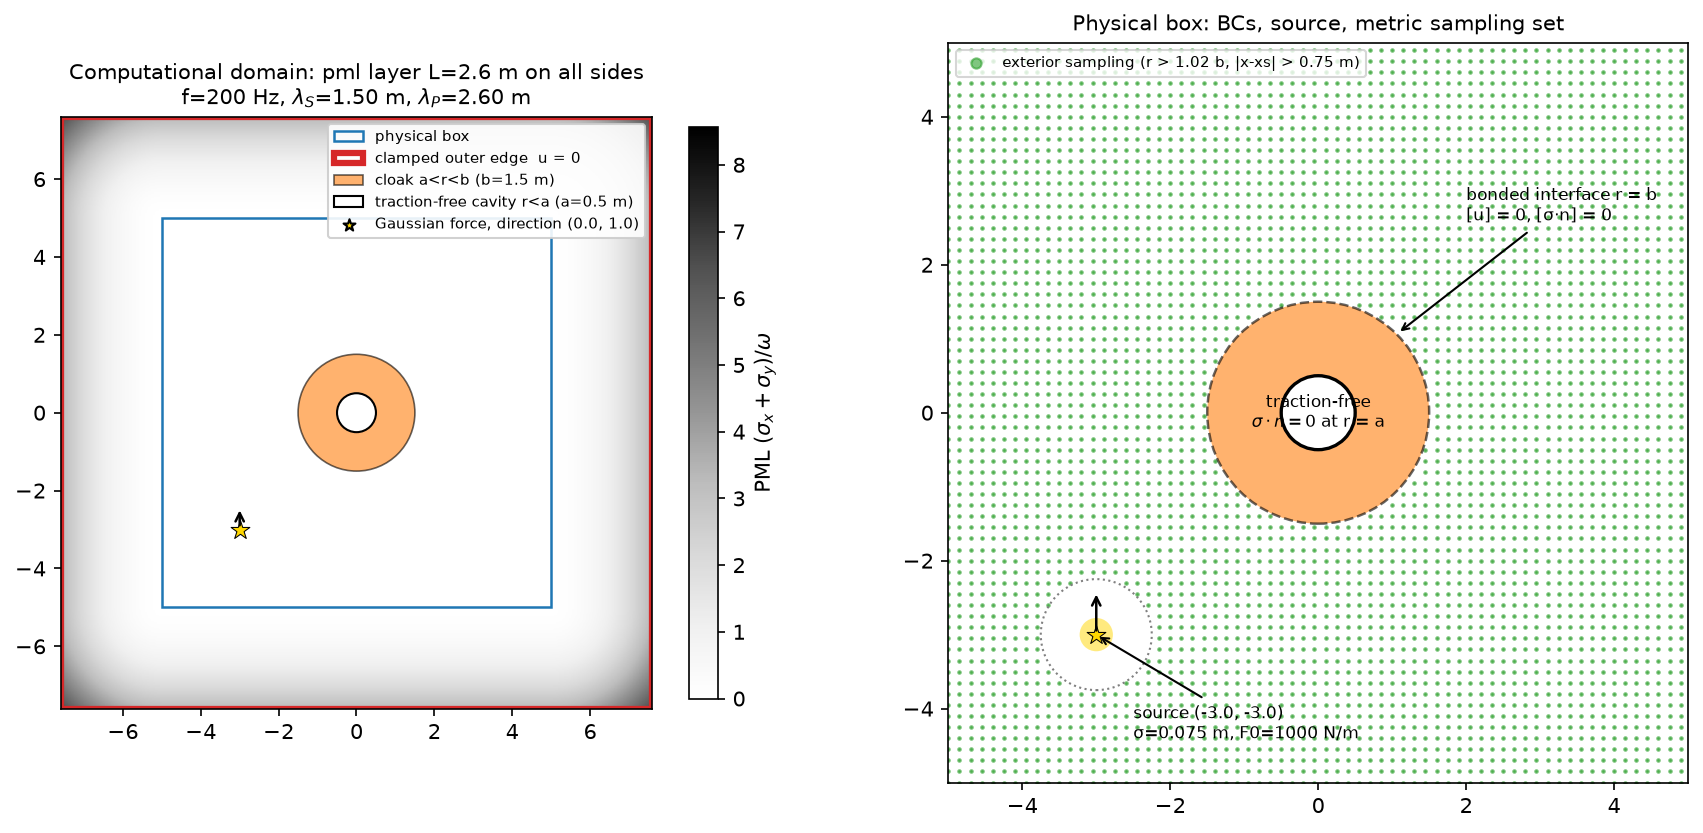
\includegraphics[width=\textwidth]{01_setup_bc_source.png}
\caption{Geometry, boundary conditions, source and sampling points, for source $(-3,-3)$\,m and vertical
force. Left: the full domain with the PML stretching $(\sigma_x+\sigma_y)/\omega$. Right: the physical box with
exterior sampling points (a subset, plotted at 0.15\,m spacing) and the excluded source neighbourhood. The label $\sigma$ in the right panel is the Gaussian width $w$ of~\eqref{eq:source}.}
\label{fig:setup}
\end{figure}

%% =============================================================
\section{The regularised cloak}\label{sec:cloak}
%% =============================================================

\subsection{Radial maps}

Let $\Xi$ map the virtual annulus $\varepsilon\le R\le b$ onto the physical annulus $a\le r\le b$ radially,
$r=\phi(R)$, $\theta=\Theta$, with $0<\varepsilon<a<b$, and let $\Xi$ be the identity for $R\ge b$. We use the linear
and quadratic maps of~\citet[Appendix]{chatzopoulos2023},
\begin{align}
  \phi_{1}(R)&=a+\frac{b-a}{b-\varepsilon}\,(R-\varepsilon),\label{eq:linear}\\
  \phi_{2}(R)&=A_2R^2+A_1R+A_0,\label{eq:quadratic}\\
  A_2&=\frac{a-\varepsilon}{(b-\varepsilon)^2},\quad
  A_1=1-\frac{2b(a-\varepsilon)}{(b-\varepsilon)^2},\quad
  A_0=\frac{b^2(a-\varepsilon)}{(b-\varepsilon)^2}.\nonumber
\end{align}
Both satisfy $\phi(\varepsilon)=a$, $\phi(b)=b$. Also $\phi_2'(b)=1$, and $\phi_2$ is increasing on
$[\varepsilon,b]$ if and only if $b-\varepsilon>2(a-\varepsilon)$, as $\phi_2'(\varepsilon)=1-2(a-\varepsilon)/(b-\varepsilon)$.
The base case is $\phi_1$ with $\varepsilon=0.005$\,m.

Because $\theta=\Theta$, the polar frames at $\mbf{X}$ and $\mbf{x}$ coincide, and the transformation gradient
$\mbf{F}=\partial\mbf{x}/\partial\mbf{X}$ is
\be\label{eq:F}
  \mbf{F}=F_r\,\er\otimes\er+F_\theta\,\et\otimes\et,\qquad
  F_r=\phi'(R),\quad F_\theta=\frac{r}{R},\quad J=\det\mbf{F}=F_rF_\theta .
\ee

\subsection{The transformed medium}

With the gauge $\mbf{U}(\mbf{X})=\mbf{u}(\mbf{x})$~\citep{brun2009,norris2011}, the cloak has
\be\label{eq:pushforward}
  C'_{ijkl}=J^{-1}F_{jJ}F_{lL}\,C_{iJkL},\qquad \rho'=\rho\,J^{-1}.
\ee
This is Eq.~(5) of~\citet{chatzopoulos2023} after the index transposition $i\leftrightarrow j$, $k\leftrightarrow l$, as
that work writes the gradient on the first and third indices. The next theorem is the basis of the validation.

\begin{theorem}[Equivalence with the virtual problem]\label{thm:equivalence}
Let $0<\varepsilon<a$, and let $\Omega_\varepsilon=\Xi^{-1}(\Omega_a)$ be the truncated domain with the disk $R<\varepsilon$
removed. Assume that $\mbf{f}$ vanishes in $r<b$. Then $\mbf{U}$ solves the weak problem on $\Omega_\varepsilon$
with the background medium in $\varepsilon<R<b$ (case D) if and only if $\mbf{u}=\mbf{U}\circ\Xi^{-1}$
solves~\eqref{eq:weak} with~\eqref{eq:pushforward} in $a<r<b$ (case C). In particular:
\begin{enumerate}
\item[(i)] $\mbf{u}=\mbf{U}$ for $r\ge b$, and $\mbf{u}(\mbf{x})=\mbf{U}(\Xi^{-1}(\mbf{x}))$ for $a\le r\le b$;
\item[(ii)] the traction-free condition on $R=\varepsilon$ corresponds to the traction-free condition on $r=a$;
\item[(iii)] the traction is continuous across $r=b$ for any increasing $C^1$ map $\phi$ with $\phi(\varepsilon)=a$, $\phi(b)=b$. The condition
$\phi'(b)=1$ is not required for this, although it makes $C'$ continuous at $r=b$.
\end{enumerate}
\end{theorem}

\begin{pf}
For $\varepsilon>0$, $\Xi$ is a bi-Lipschitz homeomorphism from $\Omega_\varepsilon$ onto $\Omega_a$, since $\phi$
is $C^1$ and increasing on $[\varepsilon,b]$, $R\ge\varepsilon>0$, and it is the identity beyond $b$. Hence composition
with $\Xi^{-1}$ is a bijection of $V_\varepsilon$ onto $V_a$ preserving the clamped condition. Take $\mbf{W}\in V_\varepsilon$ and
$\mbf{w}=\mbf{W}\circ\Xi^{-1}$. The chain rule gives $\partial W_i/\partial X_J=F_{jJ}\,\partial w_i/\partial x_j$, and
$\mathrm{d}\mbf{X}=J^{-1}\mathrm{d}\mbf{x}$. Therefore, on the annulus,
\begin{align*}
\int_{\varepsilon<R<b}\! C_{iJkL}\frac{\partial U_k}{\partial X_L}\frac{\partial V_i}{\partial X_J}\,\mathrm{d}\mbf{X}
&=\int_{a<r<b}\! J^{-1}F_{jJ}F_{lL}C_{iJkL}\,\partial_l u_k\,\partial_j v_i\,\mathrm{d}\mbf{x}\\
&=\int_{a<r<b}\! C'_{ijkl}\,\partial_l u_k\,\partial_j v_i\,\mathrm{d}\mbf{x},\\
\int_{\varepsilon<R<b}\!\rho\,U_iV_i\,\mathrm{d}\mbf{X}&=\int_{a<r<b}\!\rho'\,u_iv_i\,\mathrm{d}\mbf{x}.
\end{align*}
Outside the annulus $\Xi$ is the identity and the integrands agree, including the force term, since $\mbf{f}$
vanishes in $r<b$. So the two bilinear forms and right-hand sides coincide under the bijection, which proves the
equivalence and~(i).

For the tractions, let $\Sigma_{iJ}=C_{iJkL}\partial U_k/\partial X_L$ and $\sigma'_{ij}=C'_{ijkl}\partial_lu_k$. Then
$\sigma'_{ij}=J^{-1}F_{jJ}\Sigma_{iJ}$. Nanson's formula, $n_j\,\mathrm{d}s=J\,F^{-1}_{Kj}N_K\,\mathrm{d}S$, yields
\be\label{eq:traction}
\sigma'_{ij}n_j\,\mathrm{d}s=\Sigma_{iK}N_K\,\mathrm{d}S .
\ee
Since $\mathrm{d}s=F_\theta\,\mathrm{d}S$ on circles and $F_\theta<\infty$, the traction vanishes on $r=a$ if and only if it
vanishes on $R=\varepsilon$, which is~(ii). On $r=b$ one has $F_\theta=1$, hence $\mathrm{d}s=\mathrm{d}S$
and $\sigma'_{ij}n_j=\Sigma_{iK}N_K$ from the inside. The virtual field has continuous traction across $R=b$
as the medium there is uniform, and outside $\Xi$ is the identity, which gives~(iii).\qedbox
\end{pf}

\begin{remark}
\citet{chatzopoulos2023} derive their quadratic and cubic coefficients from the requirement
$\phi'(b)=1$, described as traction continuity. In the weak formulation above, the linear map gives traction
continuity as well, with a jump of $C'$ and $\rho'$ at $r=b$. Our results for the two maps agree
(Table~\ref{tab:map}), which is consistent with both having the same virtual problem.
\end{remark}

The hypothesis on $\mbf{f}$ holds up to the Gaussian tail: the distance from each source to $r=b$ exceeds
$33w$, so $g<e^{-500}$ throughout the cloak. Theorem~\ref{thm:equivalence} is why case D is useful. The difference
C$-$D measures implementation and discretisation error, as it vanishes for the exact solutions, whereas D$-$A
is due to $\varepsilon$ alone. For $\varepsilon>0$, case C is therefore a near-cloak: a
regularised approximation to the singular limit, not a perfect cloak.

\subsection{Polar form}

\begin{proposition}\label{prop:polar}
Let $g=F_r/F_\theta$. In the orthonormal basis $(\er,\et)$, the only non-zero components of~\eqref{eq:pushforward} for the isotropic
background~\eqref{eq:C0} are
\be\label{eq:polar}
\begin{gathered}
C'_{rrrr}=g\,(\lambda+2\mu),\quad C'_{\theta\theta\theta\theta}=g^{-1}(\lambda+2\mu),\quad
C'_{rr\theta\theta}=C'_{\theta\theta rr}=\lambda,\\
C'_{r\theta r\theta}=g^{-1}\mu,\quad C'_{\theta r\theta r}=g\,\mu,\quad C'_{r\theta\theta r}=C'_{\theta rr\theta}=\mu .
\end{gathered}
\ee
The Cartesian tensor used by the solver is the full fourth-order rotation
$C'_{ijkl}=Q_{ip}Q_{jq}Q_{ks}Q_{lt}C'_{pqst}$ with $\mbf{Q}=[\er\,|\,\et]$. Moreover:
\begin{enumerate}
\item[(a)] $C'$ has major symmetry, $C'_{ijkl}=C'_{klij}$;
\item[(b)] minor symmetry holds at a point if and only if $g=1$ there; for the maps used here this occurs only at $r=b$ for $\phi_2$;
\item[(c)] for every radial map, the $2\times2$ shear block has zero determinant, and the corresponding null
gradient is the image of an infinitesimal rotation.
\end{enumerate}
\end{proposition}

\begin{pf}
In the polar basis $\mbf{F}=\mathrm{diag}(F_1,F_2)$ with $F_1=F_r$, $F_2=F_\theta$, so~\eqref{eq:pushforward}
gives $C'_{ijkl}=F_jF_lC_{ijkl}/(F_1F_2)$, without summation. As~\eqref{eq:C0} is isotropic it has the same
components in this basis, namely $C_{rrrr}=C_{\theta\theta\theta\theta}=\lambda+2\mu$, $C_{rr\theta\theta}=\lambda$,
$C_{r\theta r\theta}=C_{\theta r\theta r}=C_{r\theta\theta r}=\mu$. Substitution gives~\eqref{eq:polar}; for example,
$C'_{r\theta r\theta}=F_\theta^2\mu/(F_rF_\theta)=\mu/g$. Statement (a) follows by exchanging $(i,j)$ with $(k,l)$
in~\eqref{eq:pushforward}, using the major symmetry of $C$. For (b), $C'_{r\theta r\theta}-C'_{\theta rr\theta}=\mu(g^{-1}-1)$.
For (c), the block is $\mu\bigl(\begin{smallmatrix}g^{-1}&1\\1&g\end{smallmatrix}\bigr)$, of determinant zero. For a virtual
gradient $\mbf{G}_X$ the proof of Theorem~\ref{thm:equivalence} gives $J\,C'{:}\mbf{G}_x{:}\mbf{G}_x=C{:}\mbf{G}_X{:}\mbf{G}_X$ with
$\mbf{G}_x=\mbf{G}_X\mbf{F}^{-1}$, and the right-hand side vanishes when $\mbf{G}_X$ is skew.\qedbox
\end{pf}

For $\varepsilon=0$ and $\phi_1$ one has $g=(r-a)/r$, the form given by~\citet{nassar2018}. Dividing~\eqref{eq:polar}
by $\rho'=\rho/(F_rF_\theta)$ gives local speeds $F_rc_{P,S}$ radially and $F_\theta c_{P,S}$ tangentially, so that the local radial wavelength is $F_r\lambda_{P,S}$. Under $\phi_1$, at $r=a$ one has
$F_\theta=a/\varepsilon$, and in the base case $F_r=0.669$, $F_\theta=100$, $J=66.9$, $\rho'/\rho=0.015$ and
$C'_{\theta\theta\theta\theta}/(\lambda+2\mu)=149.5$ (Fig.~\ref{fig:material}).

The near field of the virtual hole has radial extent of order $\varepsilon$, which in physical space is a layer of thickness
\be\label{eq:delta}
  \delta=\varepsilon\,\phi'(\varepsilon)
\ee
next to the cavity. The mesh is graded accordingly (Section~\ref{sec:discretisation}).

\begin{figure}[!htb]
\centering
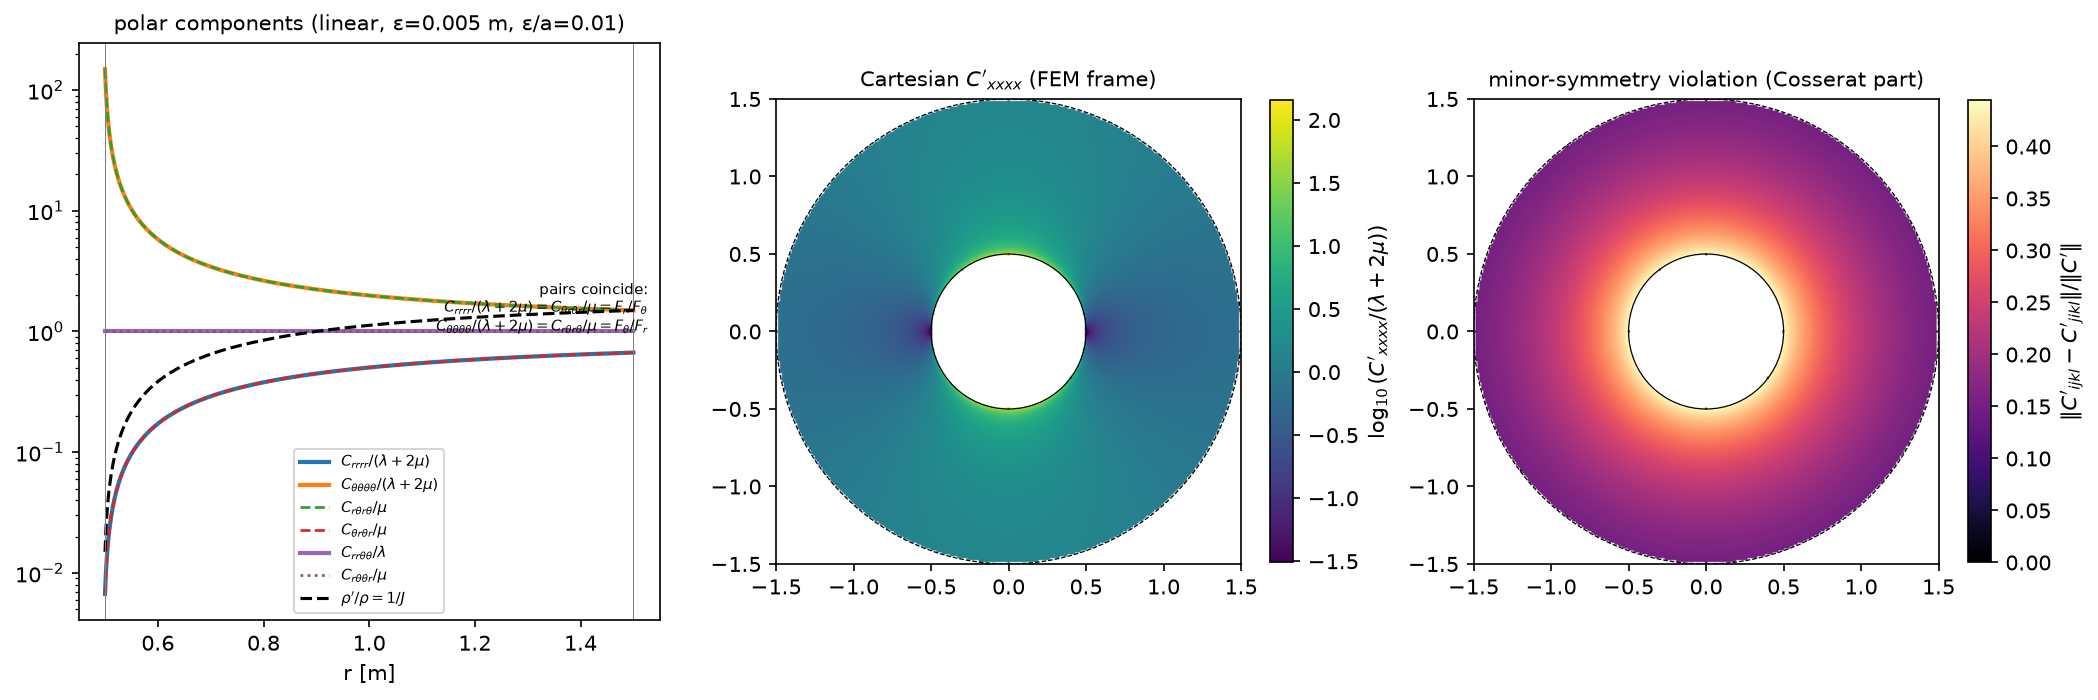
\includegraphics[width=\textwidth]{03_material.png}
\caption{Cloak material for $\phi_1$, $\varepsilon/a=0.01$. Left: polar components~\eqref{eq:polar} and $\rho'/\rho$. Centre:
Cartesian $C'_{xxxx}$. Right: relative violation of minor symmetry, $\|C'_{ijkl}-C'_{jikl}\|/\|C'\|$.}
\label{fig:material}
\end{figure}

\subsection{Scaling with $\varepsilon$: a formal estimate}\label{sec:scaling}

By Theorem~\ref{thm:equivalence}, the exterior error is the scattering of the $\varepsilon$-hole. The following is a formal estimate, not a
theorem. For $k\varepsilon\ll1$, the hole removes mass and stiffness from an area $\pi\varepsilon^2$. To
leading order, the exterior perturbation is the field of a point force proportional to
$\pi\varepsilon^2\rho\omega^2\mbf{U}^{\mathrm{inc}}(\mbf{x}_c)$ and of a force dipole proportional to
$\pi\varepsilon^2$ times the incident gradient at $\mbf{x}_c$. Both scale as $\varepsilon^2$, so we expect
$\|\mbf{u}_D-\mbf{u}_A\|=O(\varepsilon^2)$ at fixed frequency. For fixed $\varepsilon$ and $k r\gg1$, the point-force
contribution relative to the incident field is of order $(k\varepsilon)^2(kr)^{-1/2}$, that is $\propto f^{3/2}$, in view of
the far-field decay of the two-dimensional Green tensor. Both trends are compared with the computations in
Section~\ref{sec:results}.

%% =============================================================
\FloatBarrier
\section{Numerical model}\label{sec:numerics}
%% =============================================================

\subsection{Perfectly matched layer}\label{sec:pml}

Let $d_x,d_y\ge0$ be the distances into the layer along each axis, and define the stretching
\be\label{eq:stretch}
  s_j=1-\mathrm{i}\,\frac{\sigma_j(d_j)}{\omega},\qquad \sigma_j(d)=\sigma_{\max}\Bigl(\frac{d}{L}\Bigr)^{p},\qquad
  \sigma_{\max}=\frac{(p+1)\,c_P\ln(1/R)}{2L},
\ee
following the stretched-coordinate form of the PML~\citep{berenger1994,chew1994} and its elastodynamic
use~\citep{basu2003}. We use $L=2.6$\,m ($\approx\lambda_P$ at $f=200$\,Hz), $p=2$ and $R=10^{-6}$.

\begin{proposition}\label{prop:pml}
The stretched coordinates $\tilde{x}_j=x_j-\frac{\mathrm{i}}{\omega}\int_0^{d_j}\!\sigma_j\,\mathrm{d}d$ applied to the homogeneous medium
amount to the push-forward~\eqref{eq:pushforward} with the complex diagonal $\mbf{F}=\mathrm{diag}(s_x^{-1},s_y^{-1})$:
\be\label{eq:pml}
  C^{c}_{ijkl}=C_{ijkl}\,\frac{s_xs_y}{s_js_l}\quad\text{(no sum on $j,l$)},\qquad \rho^{c}=\rho\,s_xs_y .
\ee
The resulting bilinear form is complex symmetric. An outgoing plane wave at normal incidence with speed $c$ decays as
$\exp(-\int_0^{d}\sigma\,\mathrm{d}d'/c)$, independently of $\omega$. After reflection at the clamped edge, its amplitude at the
interface is the factor $\exp(-2\sigma_{\max}L/((p+1)c))$, which equals $R$ for $c=c_P$ and is smaller for $c=c_S$.
\end{proposition}

\begin{pf}
The weak form in the variables $\tilde{\mbf{x}}$ has $\partial/\partial\tilde{x}_j=s_j^{-1}\partial_j$ and
$\mathrm{d}\tilde{\mbf{x}}=s_xs_y\,\mathrm{d}\mbf{x}$, which gives~\eqref{eq:pml} directly, the same computation as
Theorem~\ref{thm:equivalence}. Symmetry of the bilinear form follows because exchanging $(i,j)$ with $(k,l)$ leaves~\eqref{eq:pml}
unchanged. With $k=\omega/c$ and the time factor $e^{+\mathrm{i}\omega t}$, an outgoing wave is $e^{-\mathrm{i}k\tilde{x}}=e^{-\mathrm{i}kx}\exp(-\int\sigma\,\mathrm{d}d'/c)$.
The integral over a round trip of the layer is $2\sigma_{\max}L/(p+1)$.\qedbox
\end{pf}

Proposition~\ref{prop:pml} concerns exact plane waves; the discrete layer can reflect more, and an oblique wave decays more slowly by the
cosine of its angle of incidence, so the layer was tested numerically (Table~\ref{tab:layers}). The formulation is also
compared with a graded damping layer, $C\to(1+\mathrm{i}\xi)C$, $\rho\to(1-\mathrm{i}\xi)\rho$, which is absorbing but not matched.

\subsection{Discretisation and solver}\label{sec:discretisation}

The weak form~\eqref{eq:weak} is discretised with isoparametric six-node triangles and a six-point quadrature rule, in real arithmetic with
four unknowns per node, using JAX-FEM~\citep{xu2020jaxfem} for assembly. The mesh is produced by Gmsh~\citep{geuzaine2009} and fragmented
into four tagged regions (disk, annulus, physical box, layer), so that the circles $r=a$ and $r=b$ are element edges with mid-side nodes on the true curve. Material is assigned
per element region and evaluated at the quadrature points, with no material pixels or cell averaging. Cases A, B and C share all nodes outside $r=a$; A retains the disk elements, and D has its own mesh with the hole at $R=\varepsilon$.

The base element sizes are $h_{\mathrm{bg}}=\lambda_S/16=0.094$\,m in the background, $h_{\mathrm{bg}}/2$ in the annulus,
$h(r{=}a)=2\delta=6.7$\,mm with $\delta$ from~\eqref{eq:delta}, graded back over $0.3$\,m, and $w/2$ at the source
(Fig.~\ref{fig:mesh}). This gives 82\,738 elements and 664\,516 real unknowns in case A. Linear systems are
factorised with MKL PARDISO, and relative residuals are at most of order $10^{-12}$. Since the matrix does not depend on the force,
one factorisation serves all force directions (Proposition~\ref{prop:superposition}).

\begin{figure}[!htb]
\centering
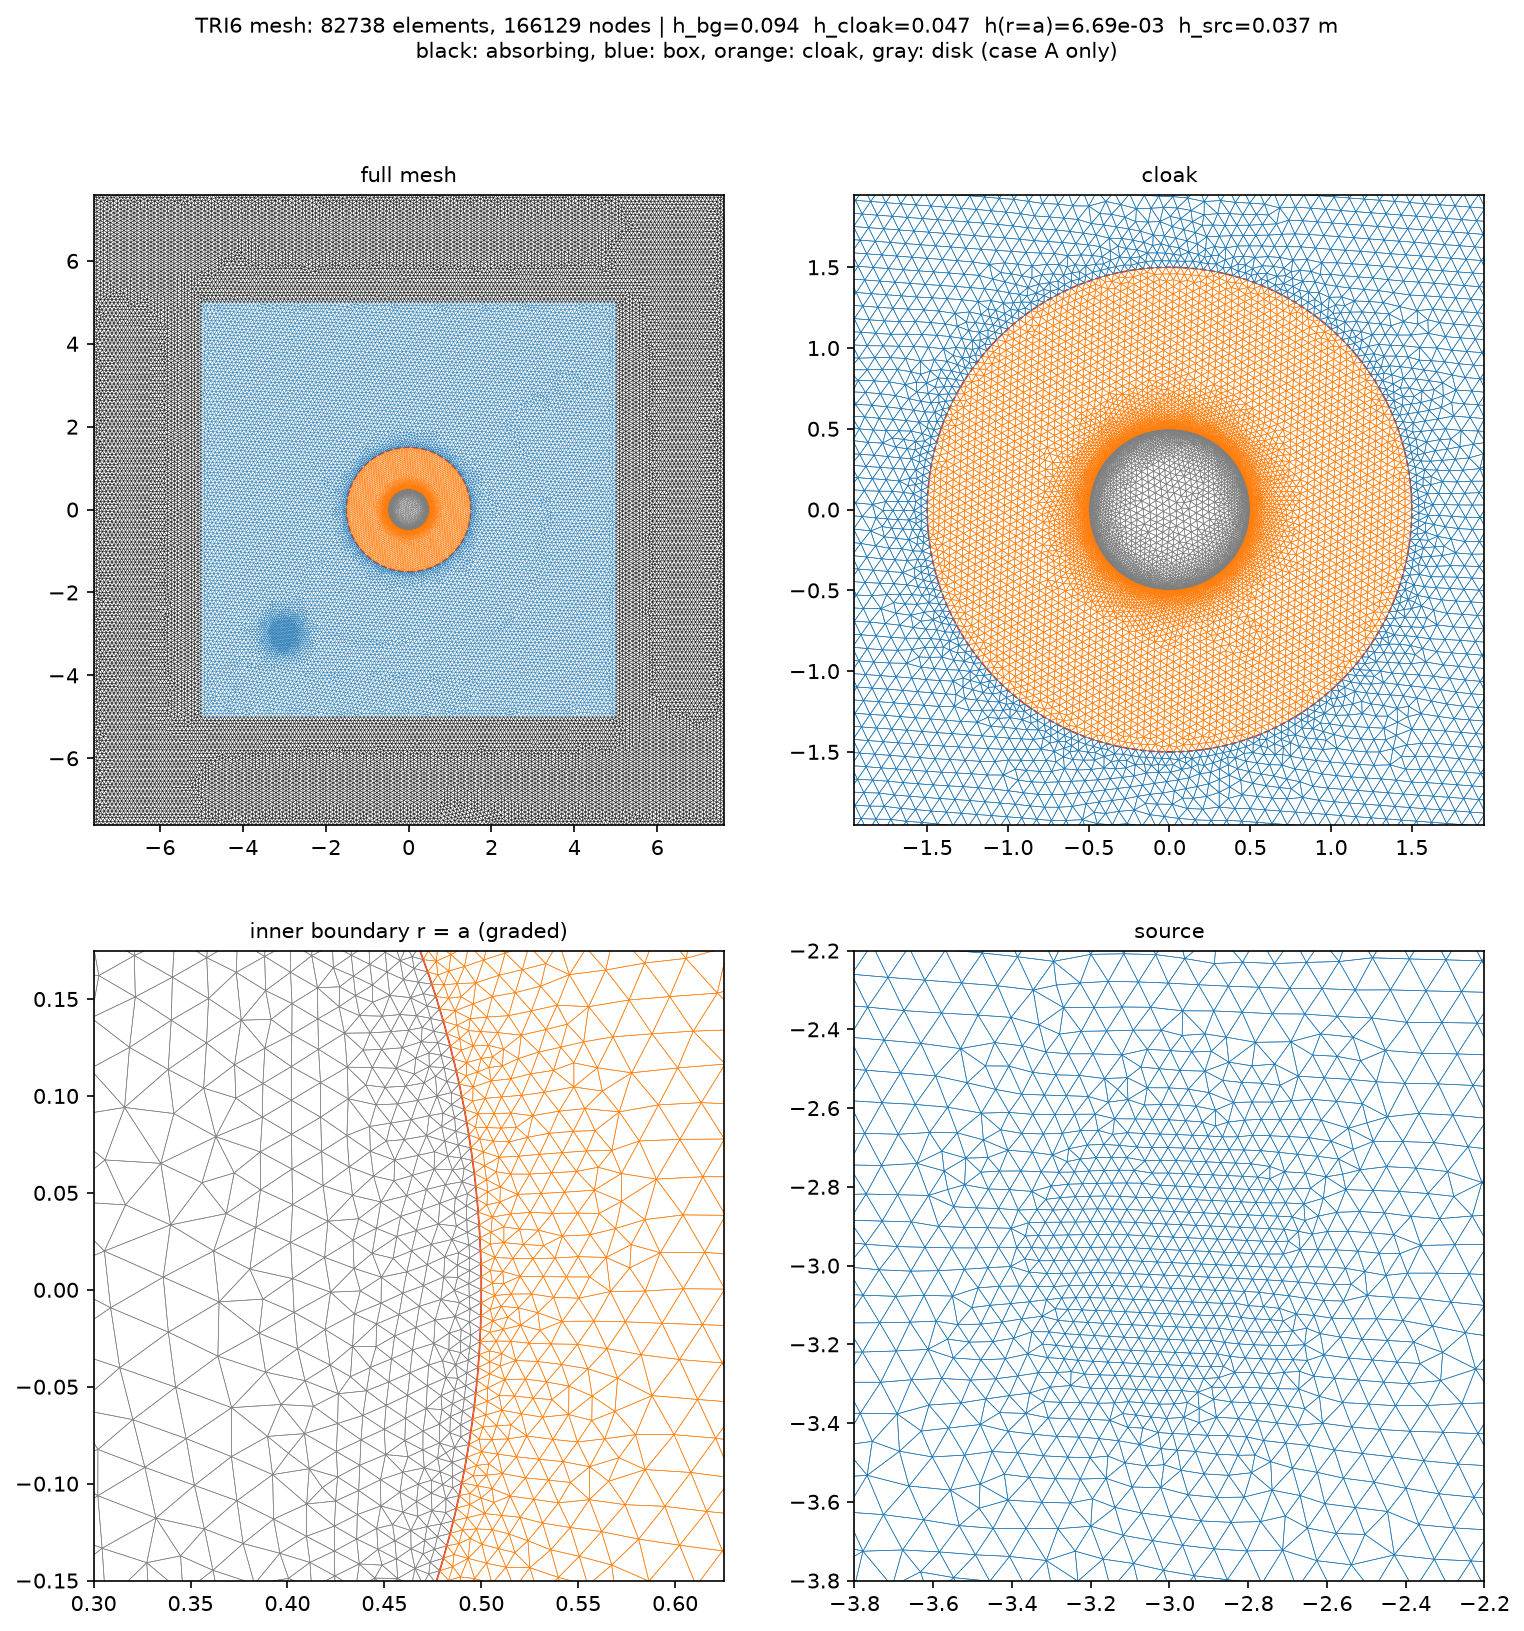
\includegraphics[width=0.82\textwidth]{02_mesh.png}
\caption{Base mesh: full domain, cloak, graded inner boundary and source neighbourhood.}
\label{fig:mesh}
\end{figure}

\subsection{Metrics}

All comparisons use a common, mesh-independent set of exterior points: a uniform grid of spacing 0.05\,m over the physical box,
keeping $r>1.02\,b$ and $\|\mbf{x}-\mbf{x}_s\|>0.75$\,m ($=\lambda_S/2$ at the base frequency), which gives 36\,747 points at $\mbf{x}_s=(-3,-3)$\,m. Fields are evaluated by exact inversion of the isoparametric map. With the total displacement
\be\label{eq:mag}
  \|\mbf{u}\|=\sqrt{|u_x|^2+|u_y|^2},
\ee
the primary metric is the normalised error in magnitude, and the secondary metric the complex displacement error:
\be\label{eq:metrics}
  e_X=\frac{\bigl\|\,\|\mbf{u}_X\|-\|\mbf{u}_A\|\,\bigr\|_{2}}{\bigl\|\,\|\mbf{u}_A\|\,\bigr\|_{2}},\qquad
  e^{c}_X=\frac{\|\mbf{u}_X-\mbf{u}_A\|_{2}}{\|\mbf{u}_A\|_{2}} .
\ee
The metric $e_X$ cannot see the phase or direction of $\mbf{u}$, whereas $e^c_X$ can. In this study $e^c_X$ is
about twice $e_X$. For frequency sweeps, we also report
\be\label{eq:eta}
  \eta_X=\frac{\langle\|\mbf{u}_X\|\rangle}{\langle\|\mbf{u}_A\|\rangle},
\ee
with averages over points beyond the cloak as seen from the source, $(\mbf{x}-\mbf{x}_c)\cdot\hat{\mbf{s}}>b$, where $\hat{\mbf{s}}$ is the unit vector
from $\mbf{x}_s$ to $\mbf{x}_c$. Then $\eta_A=1$ by definition.

\section{Verification identities}\label{sec:verification}

\begin{proposition}[Closed-form reference]\label{prop:green}
In the unbounded homogeneous medium, the solution of~\eqref{eq:strong} for the unit-integral Gaussian~\eqref{eq:source} is, up to a term
exponentially small in $\|\mbf{x}-\mbf{x}_s\|^2/w^2$,
\be\label{eq:green}
  \mbf{u}(\mbf{x})=\frac{F_0}{\mu}\Bigl[\gamma_S\,g_S\,\hat{\mbf{d}}+\frac{1}{k_S^2}\nabla\bigl(\hat{\mbf{d}}\cdot\nabla(\gamma_S\,g_S-\gamma_P\,g_P)\bigr)\Bigr],
\ee
with $g_\alpha(r_s)=-\frac{\mathrm{i}}{4}H_0^{(2)}(k_\alpha r_s)$, $r_s=\|\mbf{x}-\mbf{x}_s\|$, $k_\alpha=\omega/c_\alpha$, $\gamma_\alpha=e^{-k_\alpha^2w^2/2}$.
\end{proposition}

\begin{pf}
Note that $(\Delta+k^2)g_\alpha=-\delta$ for $k=k_\alpha$, with $H_0^{(2)}$ outgoing for $e^{+\mathrm{i}\omega t}$. Let
$\mathcal{L}\mbf{u}=\mu\Delta\mbf{u}+(\lambda+\mu)\nabla\nabla\cdot\mbf{u}+\rho\omega^2\mbf{u}$. Direct computation gives, for scalar $h$ and constant $\mbf{d}$,
\begin{align*}
  \mathcal{L}(\mbf{d}\,h)&=\mu\,\mbf{d}\,(\Delta+k_S^2)h+(\lambda+\mu)\nabla(\mbf{d}\cdot\nabla h),\\
  \mathcal{L}\nabla(\mbf{d}\cdot\nabla h)&=(\lambda+2\mu)\nabla\bigl(\mbf{d}\cdot\nabla(\Delta+k_P^2)h\bigr).
\end{align*}
Take $\mbf{G}\mbf{d}=\mu^{-1}[g_S\mbf{d}+k_S^{-2}\nabla(\mbf{d}\cdot\nabla(g_S-g_P))]$. Because $(\Delta+k_P^2)(g_S-g_P)=(k_P^2-k_S^2)g_S$ and
$(\lambda+2\mu)(k_P^2-k_S^2)=-\rho\omega^2(\lambda+\mu)/\mu=-k_S^2(\lambda+\mu)$, the gradient terms cancel, leaving
$\mathcal{L}(\mbf{G}\mbf{d})=-\mbf{d}\,\delta$. This is the Green tensor for a point force. Convolving with the Gaussian $G_w=g/(2\pi w^2)$, Graf's addition theorem gives, for $\|\mbf{y}\|<r_s$,
$H_0^{(2)}(k\|\mbf{x}-\mbf{y}\|)=\sum_nH_n^{(2)}(kr_s)J_n(k\|\mbf{y}\|)e^{\mathrm{i}n\vartheta}$, with $\vartheta$ the angle between $\mbf{x}$ and $\mbf{y}$ as seen from $\mbf{x}_s$. Radial symmetry of $G_w$ retains only $n=0$, and
$\int_0^\infty J_0(k\varrho)\,w^{-2}e^{-\varrho^2/2w^2}\varrho\,\mathrm{d}\varrho=e^{-k^2w^2/2}$ yields the factors
$\gamma_\alpha$. The tail with $\|\mbf{y}\|>r_s$ is exponentially small; at the excluded radius $r_s=0.75$\,m$=10w$ the Gaussian factor is $e^{-50}$.\qedbox
\end{pf}

\begin{proposition}[Superposition of force directions]\label{prop:superposition}
Assume that the discrete system $\mbf{K}(\omega)\mbf{U}=\mbf{P}$ is non-singular, and fix the medium and the position and shape of the source. Let $\mbf{u}_H$ and $\mbf{u}_V$ be the solutions for horizontal and vertical forces. The solution for direction $\hat{\mbf{d}}=(d_1,d_2)$ is then $\mbf{u}=d_1\mbf{u}_H+d_2\mbf{u}_V$. In particular,
$\mbf{u}_{\mathrm{both}}=(\mbf{u}_H+\mbf{u}_V)/\sqrt{2}$.
\end{proposition}

\begin{pf}
$C^c$ and $\rho^c$ in~\eqref{eq:weak} do not depend on $\mbf{u}$ and both boundary conditions are homogeneous, so the left side of~\eqref{eq:weak} is linear in $\mbf{u}$ and
$\mbf{K}$ is independent of the force. By~\eqref{eq:source}, $\mbf{f}=d_1\mbf{f}_H+d_2\mbf{f}_V$, so $\mbf{P}=d_1\mbf{P}_H+d_2\mbf{P}_V$, and $\mbf{K}^{-1}$ is linear.\qedbox
\end{pf}

The problem is linear in the force, not in the material or the frequency. Non-singularity of $\mbf{K}$ is assumed here, not proved; it is supported by the factorisations and residuals observed in all solves.

\begin{proposition}[Mirror symmetry]\label{prop:mirror}
Let $\mbf{M}=\bigl(\begin{smallmatrix}0&1\\1&0\end{smallmatrix}\bigr)$ be the reflection in $y=x$. Suppose that the box, the layer, the cavity and the cloak are mapped to themselves
by $\mbf{M}$, and that $\mbf{x}_s=\mbf{M}\mbf{x}_s$. If $\mbf{u}_V$ solves~\eqref{eq:weak} with the vertical force, then
$\mbf{u}_H(\mbf{x})=\mbf{M}\,\mbf{u}_V(\mbf{M}\mbf{x})$ solves it with the horizontal force. Hence $\|\mbf{u}_H(\mbf{x})\|=\|\mbf{u}_V(\mbf{M}\mbf{x})\|$, and averages over $\mbf{M}$-invariant sets of points coincide.
\end{proposition}

\begin{pf}
Write $(T\mbf{w})(\mbf{x})=\mbf{M}\mbf{w}(\mbf{M}\mbf{x})$. Then $T$ is a bijection of $V_a$ with gradient
$\nabla(T\mbf{w})(\mbf{x})=\mbf{M}(\nabla\mbf{w})(\mbf{M}\mbf{x})\mbf{M}$. The medium is covariant:
\[C^c_{ijkl}(\mbf{M}\mbf{x})=M_{ip}M_{jq}M_{ks}M_{lt}C^c_{pqst}(\mbf{x}),\qquad \rho^c(\mbf{M}\mbf{x})=\rho^c(\mbf{x}).\]
Indeed~\eqref{eq:C0} is invariant, $\mbf{F}(\mbf{M}\mbf{x})=\mbf{M}\mbf{F}(\mbf{x})\mbf{M}$ for radial maps, and $\mbf{M}$ exchanges
$s_x$ and $s_y$ in~\eqref{eq:pml}. Changing variables $\mbf{x}\to\mbf{M}\mbf{x}$ in~\eqref{eq:weak}, of unit Jacobian modulus, shows that the bilinear form is invariant under $T$. On the right side, $g(\mbf{M}\mbf{x})=g(\mbf{x})$ and $\mbf{M}(0,1)^{T}=(1,0)^{T}$.\qedbox
\end{pf}

Hence at $\mbf{x}_s=(-3,-3)$\,m, vertical and horizontal forces give the same scalar metrics up to mesh asymmetry; they are not independent tests.
The source $(-3.5,-2)$\,m removes this symmetry.

%% =============================================================
\section{Results}\label{sec:results}
%% =============================================================

\subsection{Verification}

Case A agrees with the closed form~\eqref{eq:green} to $e=5.0\times10^{-5}$ and $e^c=2.5\times10^{-4}$ on the base mesh, and refinement gives an observed order of about $3.3$ with no floor down to the finest level (Table~\ref{tab:mesh}).
The sign of the force and the time convention are thereby confirmed. Superposition (Proposition~\ref{prop:superposition}) holds to round-off: the separately computed solve with $\hat{\mbf{d}}=(1,1)/\sqrt{2}$ equals $(\mbf{u}_V+\mbf{u}_H)/\sqrt{2}$ with $e^c$ between $1.4\times10^{-14}$ and $9.0\times10^{-14}$ over cases A--D and both source positions. Mirror symmetry (Proposition~\ref{prop:mirror}) is satisfied to $e^c=2.6\times10^{-4}$, the same order as the mesh error of case A, as expected from a non-symmetric mesh.
The material was checked independently: the closed form~\eqref{eq:F} against automatic differentiation of the map, the Cartesian tensor against the rotated form~\eqref{eq:polar}, the symmetries of Proposition~\ref{prop:polar}, invariance of the strain energy for random non-symmetric gradients, and the $\varepsilon=0$ form of~\citet{nassar2018}.

\subsection{Base case}

Table~\ref{tab:base} and Figs.~\ref{fig:fields}--\ref{fig:lines} give the base case with vertical force at $f=200$\,Hz, where $\lambda_S=1.5$\,m$=b$ and $\lambda_P=2.6$\,m. The bare hole produces strong scattering, $e=0.158$, with a low-amplitude shadow behind the cavity. In the cloak case, the magnitude agrees with case A outside $r=b$ to $e=6.7\times10^{-5}$, which is about 2400 times smaller. The two terms in the decomposition suggested by Theorem~\ref{thm:equivalence} are D vs.\ A at $7.7\times10^{-5}$ and C vs.\ D at $1.2\times10^{-5}$: the residual is dominated by the regularisation, not by the numerics.
The mapped interior comparison, of $\mbf{u}_C(\mbf{x})$ with $\mbf{u}_D(\Xi^{-1}(\mbf{x}))$, confirms part (i) of the theorem within the annulus, at $4.6\times10^{-5}$.

\begin{table}[!htb]
\centering\small
\caption{Base case: $\varepsilon/a=0.01$, linear map, vertical force, source $(-3,-3)$\,m, $f=200$\,Hz. Errors defined in~\eqref{eq:metrics}.}
\label{tab:base}
\begin{tabular}{lcc}
\toprule
Comparison & $e$ (magnitude) & $e^{c}$ (complex) \\
\midrule
B: hole without cloak vs.\ A & $1.58\times 10^{-1}$ & $3.12\times 10^{-1}$ \\
C: regularised cloak vs.\ A & $6.68\times 10^{-5}$ & $1.30\times 10^{-4}$ \\
\quad C vs.\ A on the ring $r=1.25\,b$ & $1.01\times 10^{-4}$ & $1.85\times 10^{-4}$ \\
\quad C vs.\ A on the ring $r=2\,b$ & $7.68\times 10^{-5}$ & $1.38\times 10^{-4}$ \\
D: $\varepsilon$-hole vs.\ A & $7.67\times 10^{-5}$ & $1.51\times 10^{-4}$ \\
C vs.\ D, exterior & $1.18\times 10^{-5}$ & $2.61\times 10^{-5}$ \\
$\mathbf{u}_C(\mathbf{x})$ vs.\ $\mathbf{u}_D(\Xi^{-1}(\mathbf{x}))$, annulus & $4.65\times 10^{-5}$ & $1.25\times 10^{-4}$ \\
A vs.\ closed form, Eq.~\eqref{eq:green} & $5.00\times 10^{-5}$ & $2.49\times 10^{-4}$ \\
\bottomrule
\end{tabular}

\end{table}

\begin{figure}[!htb]
\centering
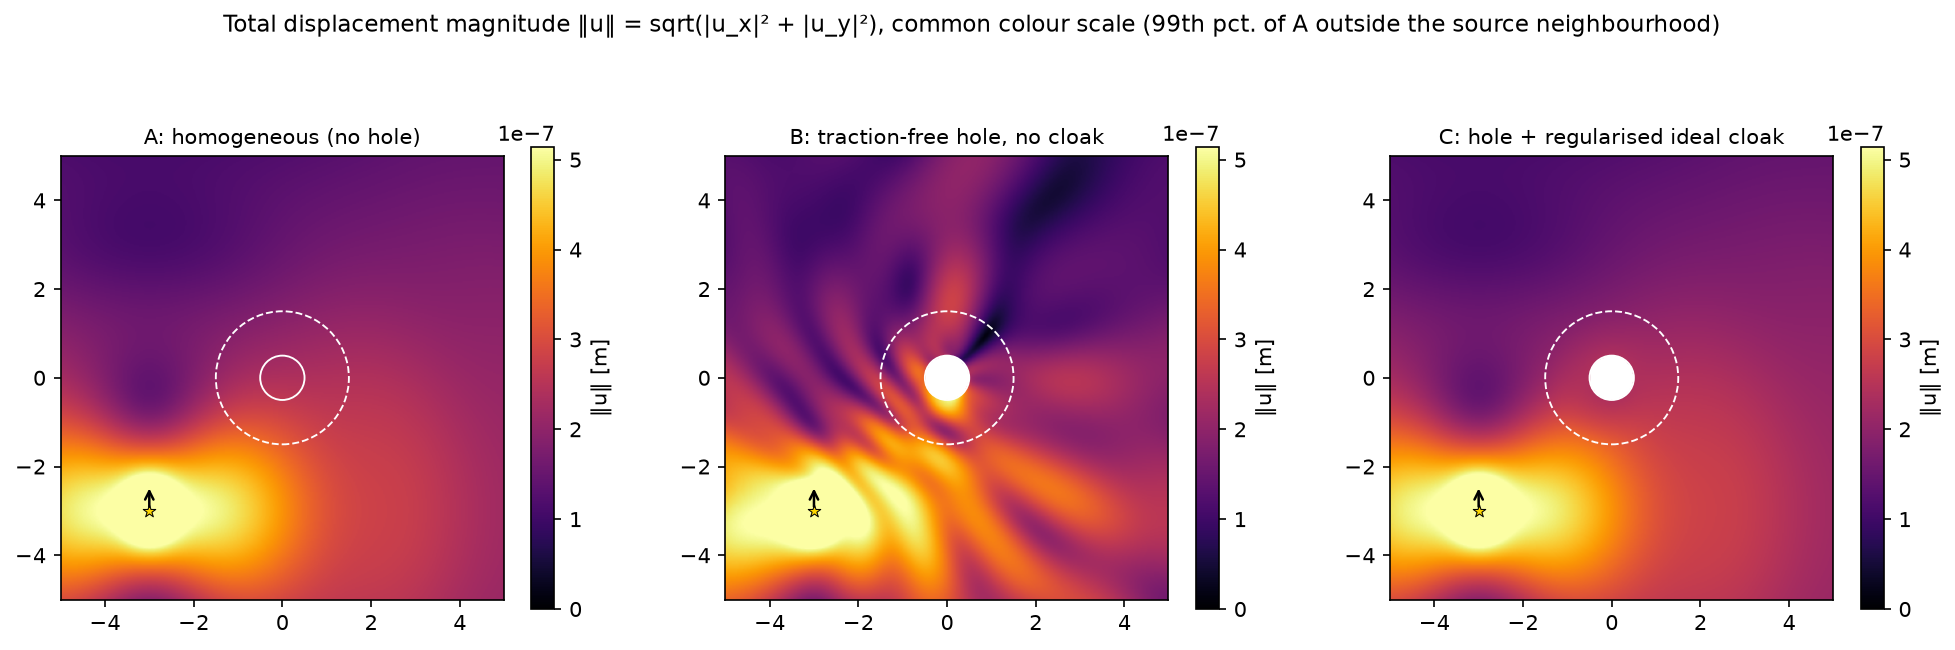
\includegraphics[width=\textwidth]{04_fields_ABC.png}
\caption{Total displacement magnitude~\eqref{eq:mag} for cases A, B and C on a common colour scale. Base case.}
\label{fig:fields}
\end{figure}

\begin{figure}[!htb]
\centering
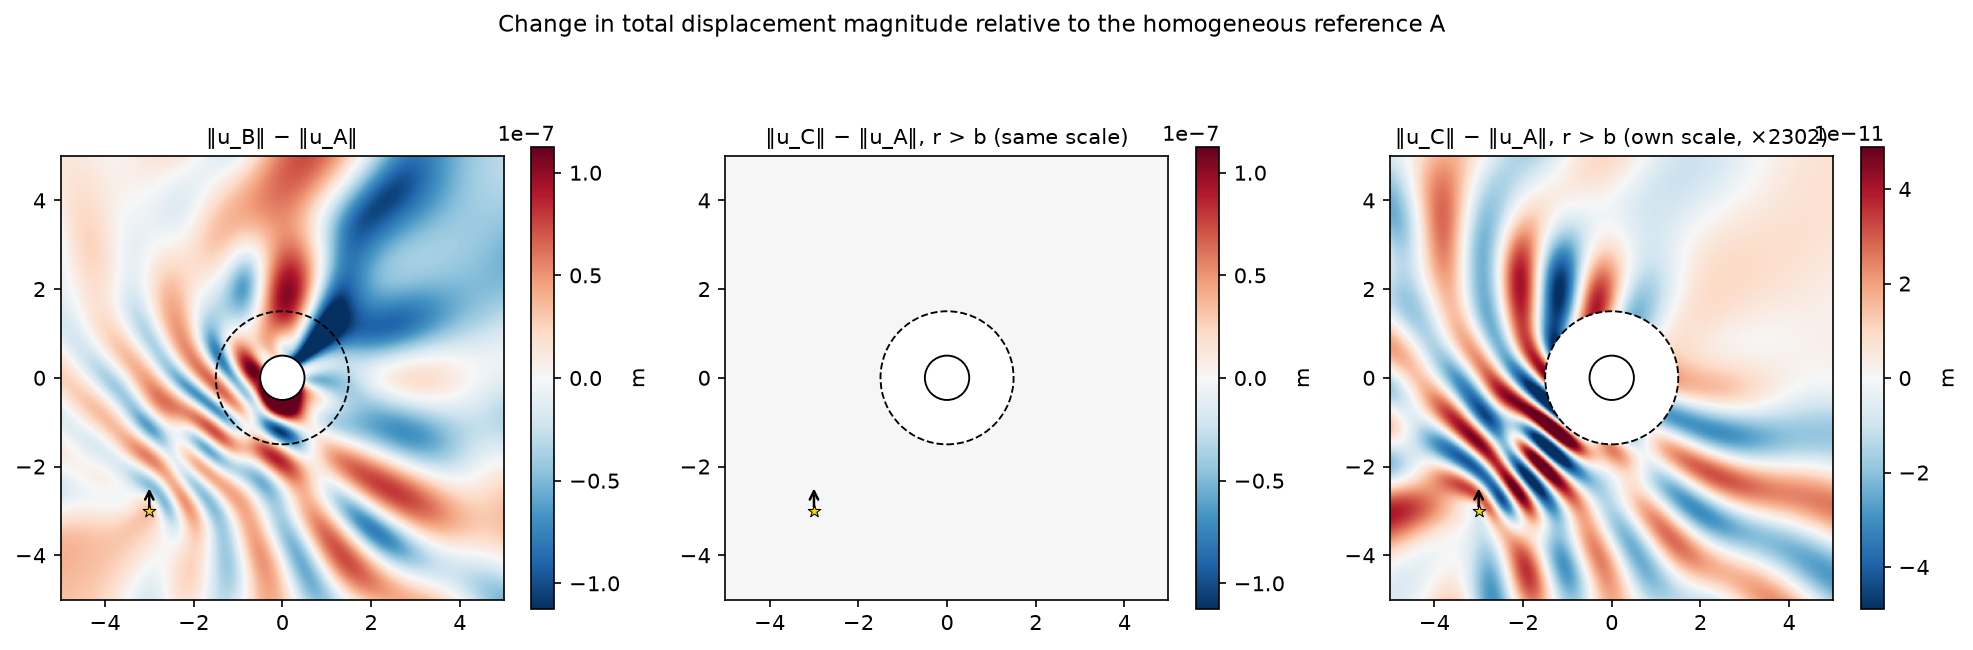
\includegraphics[width=\textwidth]{05_scattered.png}
\caption{Change in magnitude relative to case A. Left: bare hole. Centre: cloak on the same scale, masked for $r<b$, where the field is the transformed one. Right: cloak on its own scale.}
\label{fig:scattered}
\end{figure}

\begin{figure}[!htb]
\centering
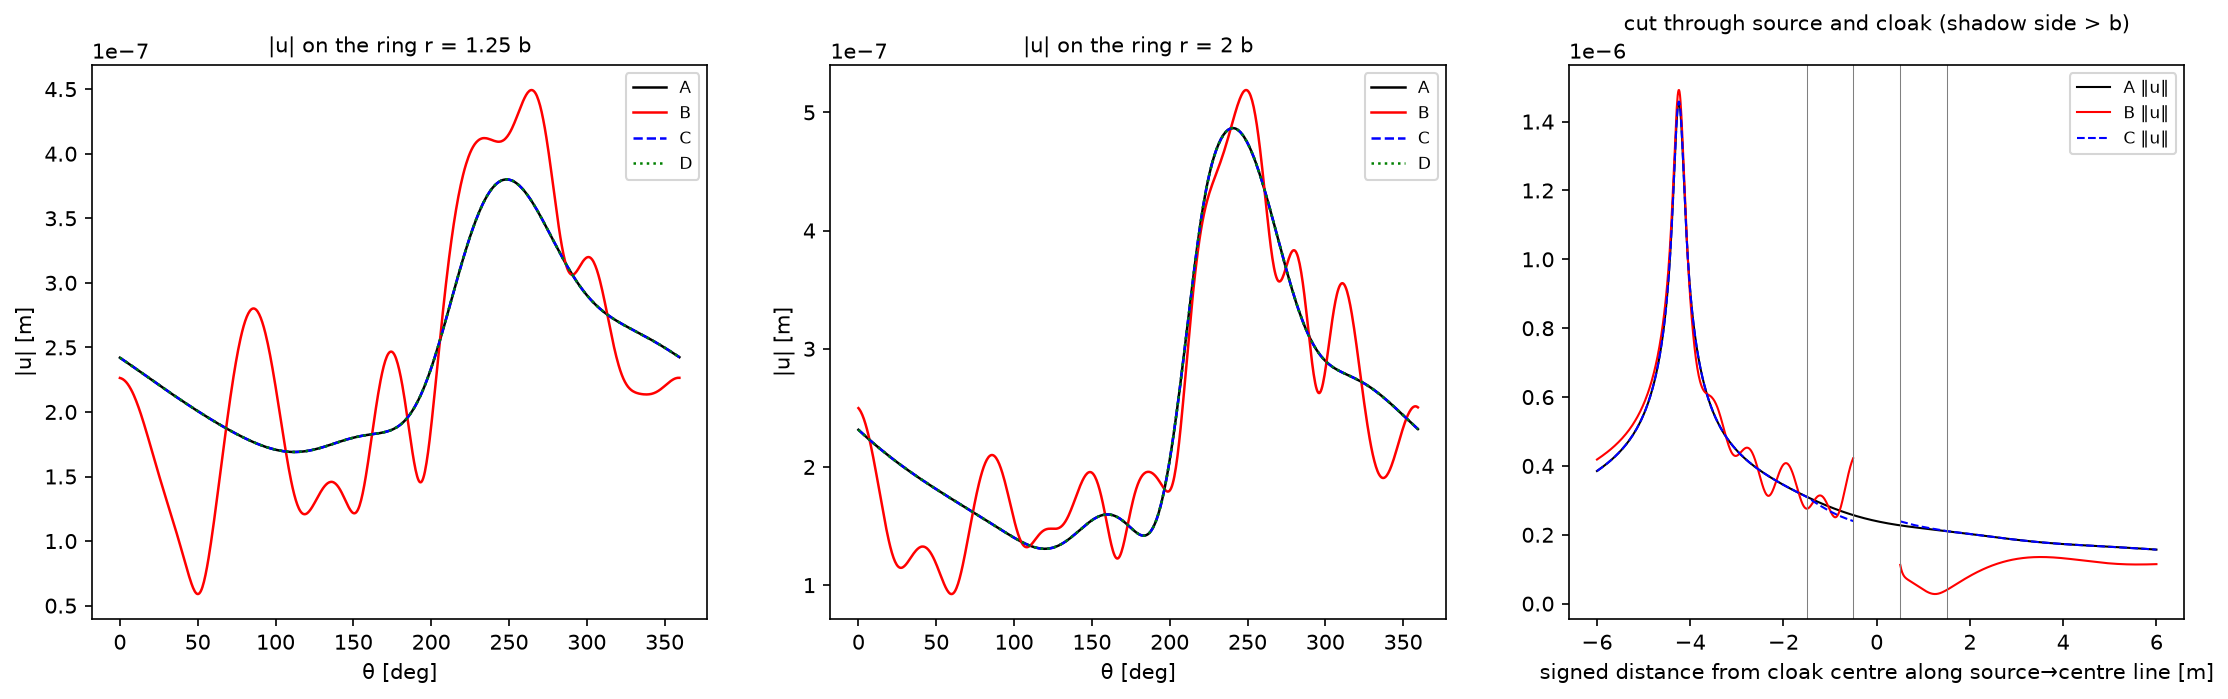
\includegraphics[width=\textwidth]{06_lines.png}
\caption{Magnitude on the rings $r=1.25\,b$ and $r=2\,b$, and along the line through source and cloak. On the rings, C and D overlap A; on the line, C leaves A only inside $r<b$.}
\label{fig:lines}
\end{figure}

\FloatBarrier
\subsection{Convergence in the regularisation}

Table~\ref{tab:eps} and Fig.~\ref{fig:eps} show the sweep in $\varepsilon$, with $h(r{=}a)$ following~\eqref{eq:delta} below a cap of 20\,mm. Between consecutive levels, D vs.\ A has observed slopes of $1.98$--$2.02$ in $\varepsilon$, in agreement with the estimate of Section~\ref{sec:scaling}. Case C follows D, and at the smallest value $\varepsilon/a=0.005$ the error is $1.6\times10^{-5}$. C vs.\ D stays between $5\times10^{-6}$ and $1.2\times10^{-4}$ but is not monotone in $\varepsilon$, because the mesh near the cavity changes along the sweep. Results at finite $\varepsilon$ approximate the ideal limit; the case $\varepsilon=0$ itself was not computed.

\begin{table}[!htb]
\centering\footnotesize
\caption{Convergence in the regularisation. Magnitude errors $e$ except for the last column. ``Interior'' compares $\mbf{u}_C(\mbf{x})$ with $\mbf{u}_D(\Xi^{-1}(\mbf{x}))$ in the annulus.}
\label{tab:eps}
\resizebox{\textwidth}{!}{\begin{tabular}{ccccccc}
\toprule
$\varepsilon/a$ & $h(r{=}a)$ [mm] & C vs.\ A & D vs.\ A & C vs.\ D & interior & C vs.\ A, $e^{c}$ \\
\midrule
0.2 & 20.0 & $3.12\times 10^{-2}$ & $3.11\times 10^{-2}$ & $1.21\times 10^{-4}$ & $3.38\times 10^{-4}$ & $6.27\times 10^{-2}$ \\
0.1 & 20.0 & $7.87\times 10^{-3}$ & $7.87\times 10^{-3}$ & $5.34\times 10^{-6}$ & $3.67\times 10^{-5}$ & $1.56\times 10^{-2}$ \\
0.05 & 20.0 & $1.88\times 10^{-3}$ & $1.94\times 10^{-3}$ & $5.78\times 10^{-5}$ & $1.86\times 10^{-4}$ & $3.72\times 10^{-3}$ \\
0.02 & 13.4 & $2.83\times 10^{-4}$ & $3.07\times 10^{-4}$ & $2.74\times 10^{-5}$ & $1.00\times 10^{-4}$ & $5.55\times 10^{-4}$ \\
0.01 & 6.7 & $6.68\times 10^{-5}$ & $7.67\times 10^{-5}$ & $1.18\times 10^{-5}$ & $4.65\times 10^{-5}$ & $1.30\times 10^{-4}$ \\
0.005 & 3.3 & $1.62\times 10^{-5}$ & $1.91\times 10^{-5}$ & $5.05\times 10^{-6}$ & $2.12\times 10^{-5}$ & $3.14\times 10^{-5}$ \\
\bottomrule
\end{tabular}
}
\end{table}

\begin{figure}[!htb]
\centering
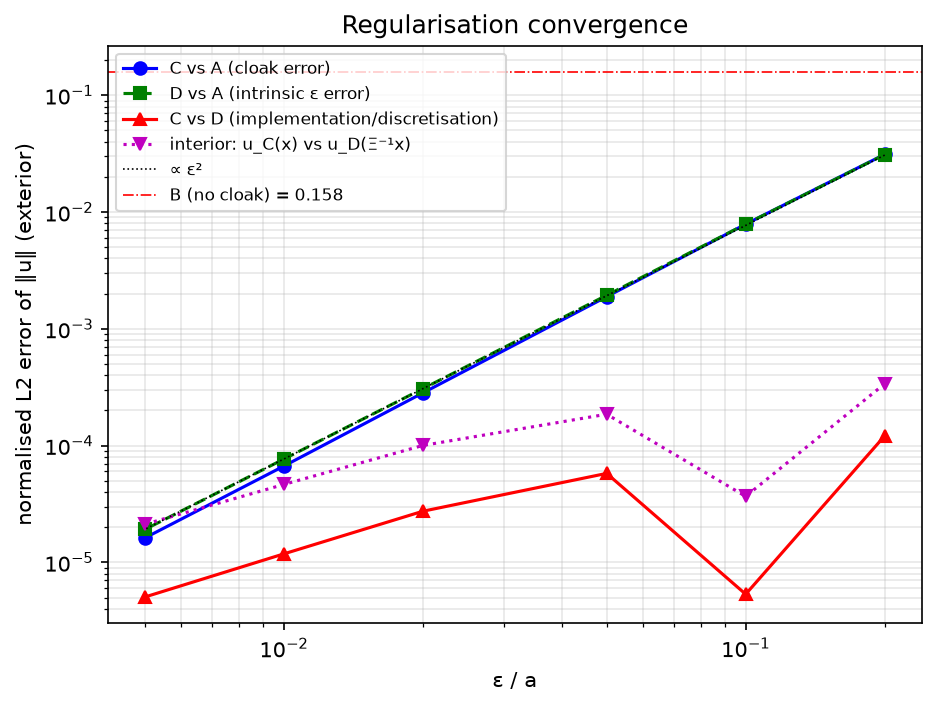
\includegraphics[width=0.62\textwidth]{07_eps_convergence.png}
\caption{Exterior error against $\varepsilon/a$, for the base case. The dotted line has slope 2.}
\label{fig:eps}
\end{figure}

\FloatBarrier
\subsection{Sensitivity to mesh, absorbing layer and radial map}

Table~\ref{tab:mesh} and Fig.~\ref{fig:meshconv} scale all element sizes together. C vs.\ A saturates at the regularisation error from about 11 elements per $\lambda_S$. C vs.\ D decreases with refinement, from $4.8\times10^{-5}$ to $9.6\times10^{-6}$, but its rate falls on the finest levels, so that we cannot state from these data whether it continues to converge at the same rate. Refinement at $r=a$ and quadrature order were not varied separately.

\begin{table}[!htb]
\centering\footnotesize
\caption{Mesh sensitivity with all sizes scaled together. Magnitude errors $e$.}
\label{tab:mesh}
\resizebox{\textwidth}{!}{\begin{tabular}{ccccccc}
\toprule
$\lambda_S/h_{\mathrm{bg}}$ & Elements & A vs.\ closed form & A vs.\ finest & C vs.\ A & D vs.\ A & C vs.\ D \\
\midrule
8.0 & 21\,562 & $4.84\times 10^{-4}$ & $4.78\times 10^{-4}$ & $7.51\times 10^{-5}$ & $7.46\times 10^{-5}$ & $4.76\times 10^{-5}$ \\
11.4 & 43\,022 & $1.52\times 10^{-4}$ & $1.47\times 10^{-4}$ & $6.58\times 10^{-5}$ & $7.62\times 10^{-5}$ & $1.84\times 10^{-5}$ \\
16.0 & 82\,738 & $5.00\times 10^{-5}$ & $4.70\times 10^{-5}$ & $6.68\times 10^{-5}$ & $7.67\times 10^{-5}$ & $1.18\times 10^{-5}$ \\
21.3 & 144\,878 & $1.92\times 10^{-5}$ & ref. & $6.83\times 10^{-5}$ & $7.69\times 10^{-5}$ & $9.60\times 10^{-6}$ \\
\bottomrule
\end{tabular}
}
\end{table}

\begin{figure}[!htb]
\centering
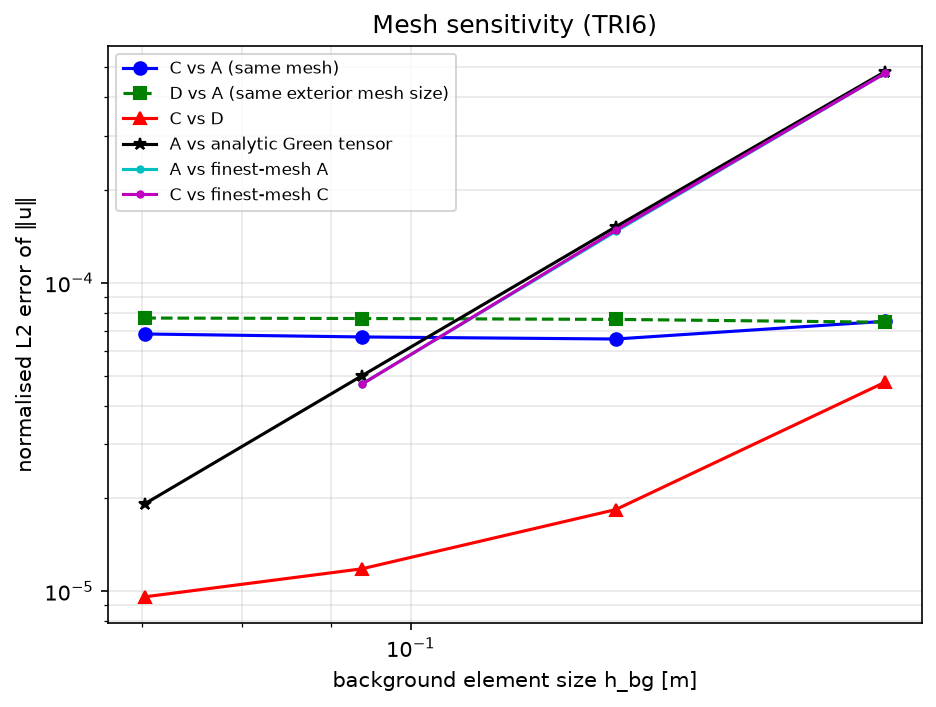
\includegraphics[width=0.62\textwidth]{08_mesh_sensitivity.png}
\caption{Magnitude errors against the background element size.}
\label{fig:meshconv}
\end{figure}

Table~\ref{tab:layers} varies the absorbing layer. The PML achieves its mesh-limited accuracy with $L\approx\lambda_P$, and is only mildly degraded at $L=1.5$\,m, $R=10^{-4}$. The damping layers are less accurate against the closed form, by a factor of about 9 for the gentler one and more than 100 for the original one, although they are longer. C vs.\ A is nearly unaffected in all cases, because A, B and C share the layer and its reflections. So that metric alone does not show the accuracy of the absolute field; the comparison with~\eqref{eq:green} does.
Table~\ref{tab:map} confirms that linear and quadratic maps perform alike, in line with Theorem~\ref{thm:equivalence}.

\begin{table}[!htb]
\centering\footnotesize
\caption{Absorbing-layer sensitivity, at $\varepsilon/a=0.01$.}
\label{tab:layers}
\resizebox{\textwidth}{!}{\begin{tabular}{lcccc}
\toprule
Layer & Elements & A vs.\ closed form, $e$ & A vs.\ closed form, $e^{c}$ & C vs.\ A, $e$ \\
\midrule
PML, $L=2.6$\,m, $R=10^{-6}$, $p=2$ (base) & 82\,738 & $5.00\times 10^{-5}$ & $2.49\times 10^{-4}$ & $6.68\times 10^{-5}$ \\
PML, $L=1.5$\,m, $R=10^{-4}$, $p=2$ & 66\,080 & $1.08\times 10^{-4}$ & $3.04\times 10^{-4}$ & $6.71\times 10^{-5}$ \\
PML, $L=4$\,m, $R=10^{-6}$, $p=2$ & 107\,256 & $5.01\times 10^{-5}$ & $2.50\times 10^{-4}$ & $6.71\times 10^{-5}$ \\
PML, $L=2.6$\,m, $R=10^{-4}$, $p=2$ & 82\,738 & $6.60\times 10^{-5}$ & $2.61\times 10^{-4}$ & $6.68\times 10^{-5}$ \\
PML, $L=2.6$\,m, $R=10^{-8}$, $p=2$ & 82\,738 & $4.99\times 10^{-5}$ & $2.49\times 10^{-4}$ & $6.68\times 10^{-5}$ \\
PML, $L=2.6$\,m, $R=10^{-6}$, $p=3$ & 82\,738 & $5.01\times 10^{-5}$ & $2.48\times 10^{-4}$ & $6.68\times 10^{-5}$ \\
damping, $L=4$\,m, $\xi_{\max}=4$, $p=2$ & 107\,256 & $1.79\times 10^{-2}$ & $3.52\times 10^{-2}$ & $6.64\times 10^{-5}$ \\
damping, $L=6$\,m, $\xi_{\max}=1.5$, $p=3$ & 149\,054 & $4.43\times 10^{-4}$ & $7.42\times 10^{-4}$ & $6.71\times 10^{-5}$ \\
\bottomrule
\end{tabular}
}
\end{table}

\begin{table}[!htb]
\centering\small
\caption{Radial maps, at $\varepsilon/a=0.01$. Magnitude errors $e$.}
\label{tab:map}
\begin{tabular}{lccc}
\toprule
Radial map & C vs.\ A & D vs.\ A & C vs.\ D \\
\midrule
linear & $6.68\times 10^{-5}$ & $7.67\times 10^{-5}$ & $1.18\times 10^{-5}$ \\
quadratic & $6.38\times 10^{-5}$ & $7.67\times 10^{-5}$ & $1.47\times 10^{-5}$ \\
\bottomrule
\end{tabular}

\end{table}

\FloatBarrier
\subsection{Force direction and source position}

Table~\ref{tab:forces} compares all forces at both source positions. At $(-3,-3)$\,m, vertical and horizontal coincide, as Proposition~\ref{prop:mirror} requires. At $(-3.5,-2)$\,m they are different problems, with bare-hole errors of $0.188$ and $0.129$, and the cloak reduces the error by a similar factor in each (Fig.~\ref{fig:offdiag}). The factor B/C lies between about 2360 and 3110 across the six cases.

\begin{table}[!htb]
\centering\footnotesize
\caption{Force direction and source position, at $\varepsilon/a=0.01$, $f=200$\,Hz. Magnitude errors $e$.}
\label{tab:forces}
\resizebox{\textwidth}{!}{\begin{tabular}{ccccccc}
\toprule
Source & Force & B vs.\ A & C vs.\ A & D vs.\ A & C vs.\ D & B/C \\
\midrule
$(-3,-3)$ & vertical & 0.158 & $6.68\times 10^{-5}$ & $7.67\times 10^{-5}$ & $1.18\times 10^{-5}$ & 2367 \\
$(-3,-3)$ & horizontal & 0.158 & $6.67\times 10^{-5}$ & $7.67\times 10^{-5}$ & $1.19\times 10^{-5}$ & 2373 \\
$(-3,-3)$ & $(1,1)/\sqrt{2}$ & 0.104 & $3.36\times 10^{-5}$ & $3.77\times 10^{-5}$ & $5.12\times 10^{-6}$ & 3110 \\
$(-3.5,-2)$ & vertical & 0.188 & $7.95\times 10^{-5}$ & $9.12\times 10^{-5}$ & $1.40\times 10^{-5}$ & 2361 \\
$(-3.5,-2)$ & horizontal & 0.129 & $5.36\times 10^{-5}$ & $6.13\times 10^{-5}$ & $8.99\times 10^{-6}$ & 2414 \\
$(-3.5,-2)$ & $(1,1)/\sqrt{2}$ & 0.111 & $4.02\times 10^{-5}$ & $4.55\times 10^{-5}$ & $6.24\times 10^{-6}$ & 2759 \\
\bottomrule
\end{tabular}
}
\end{table}

\begin{figure}[!htb]
\centering
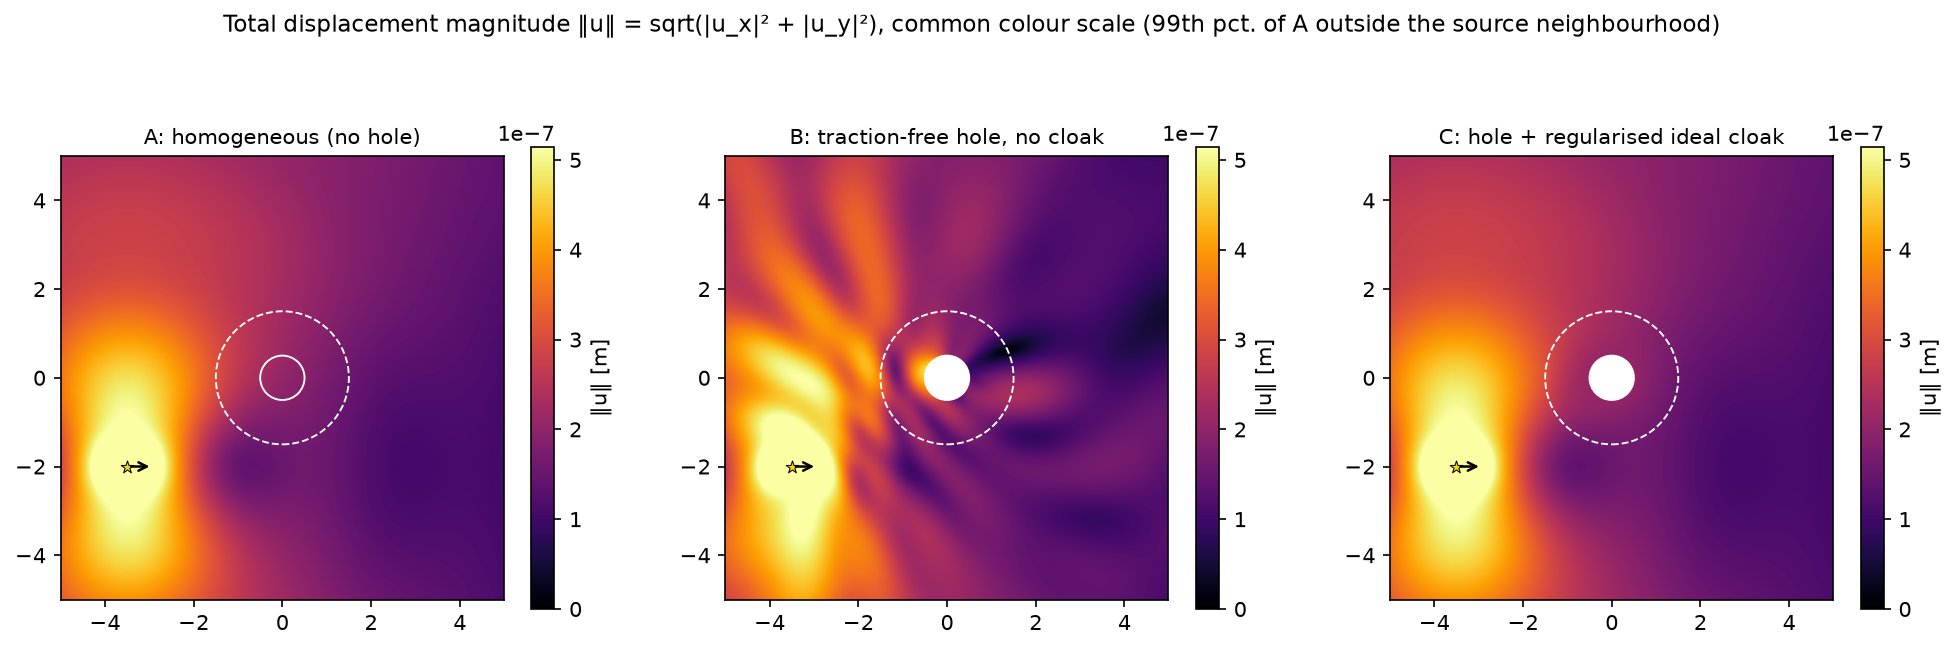
\includegraphics[width=\textwidth]{offdiag_horizontal_fields.png}
\caption{Total displacement magnitude for the source $(-3.5,-2)$\,m and horizontal force.}
\label{fig:offdiag}
\end{figure}

\FloatBarrier
\subsection{Frequency sweep}

Figures~\ref{fig:sweepratio}--\ref{fig:overview} and Table~\ref{tab:sweep} show a sweep over $f^*=bf/c_S=b/\lambda_S$ from $0.1$ to $2.5$ in steps of $0.1$ (20--500\,Hz), with $\varepsilon/a=0.01$ fixed and the six combinations of source and force, 150 in total. The background size is $h_{\mathrm{bg}}=\min(0.094\,\mathrm{m},\lambda_S/10)$, so the mesh is the base mesh up to $f^*=1.6$ and follows the wavelength above. One factorisation serves the vertical and horizontal forces, and the combined force is obtained from Proposition~\ref{prop:superposition}. At $f^*=1$ the sweep reproduces the values of Table~\ref{tab:forces} for vertical and horizontal forces.

Over the sweep, $|\eta_C-1|\le1.5\times10^{-5}$, while $e_C$ stays between $2.3\times10^{-6}$ and $3.2\times10^{-4}$ and the bare hole reaches $e_B=0.20$. For $0.5\le f^*\le1$, the observed exponent of $e_C$ with frequency lies between $1.3$ and $1.5$, close to the estimate of Section~\ref{sec:scaling}. Above about $f^*=1$, $e_C$ is of the same size as the mesh error of case A (at most $2.3\times10^{-4}$ in magnitude), so these data do not separate its growth with frequency from mesh error.

\begin{table}[!htb]
\centering\footnotesize
\caption{Selected points of the sweep, for source $(-3.5,-2)$\,m; V and H denote vertical and horizontal forces. Magnitude errors $e$, and ratio $\eta_B$ from~\eqref{eq:eta}. In all these cases $\eta_C$ differs from 1 by less than $1.6\times10^{-5}$.}
\label{tab:sweep}
\resizebox{\textwidth}{!}{\begin{tabular}{cccccccc}
\toprule
$f^*$ & $f$ [Hz] & $\eta_B$ (V) & B vs.\ A (V) & C vs.\ A (V) & $\eta_B$ (H) & B vs.\ A (H) & C vs.\ A (H) \\
\midrule
0.1 & 20 & 0.983 & 0.027 & $2.3\times 10^{-6}$ & 0.985 & 0.038 & $3.1\times 10^{-6}$ \\
0.4 & 80 & 0.902 & 0.162 & $1.9\times 10^{-5}$ & 0.972 & 0.119 & $1.5\times 10^{-5}$ \\
0.5 & 100 & 0.869 & 0.170 & $2.7\times 10^{-5}$ & 0.953 & 0.107 & $1.9\times 10^{-5}$ \\
1 & 200 & 0.854 & 0.188 & $7.9\times 10^{-5}$ & 0.876 & 0.129 & $5.4\times 10^{-5}$ \\
1.5 & 300 & 0.808 & 0.200 & $1.5\times 10^{-4}$ & 0.841 & 0.134 & $9.0\times 10^{-5}$ \\
2 & 400 & 0.821 & 0.200 & $2.2\times 10^{-4}$ & 0.840 & 0.138 & $1.5\times 10^{-4}$ \\
2.5 & 500 & 0.800 & 0.202 & $3.2\times 10^{-4}$ & 0.825 & 0.142 & $2.0\times 10^{-4}$ \\
\bottomrule
\end{tabular}
}
\end{table}

\begin{figure}[!htb]
\centering
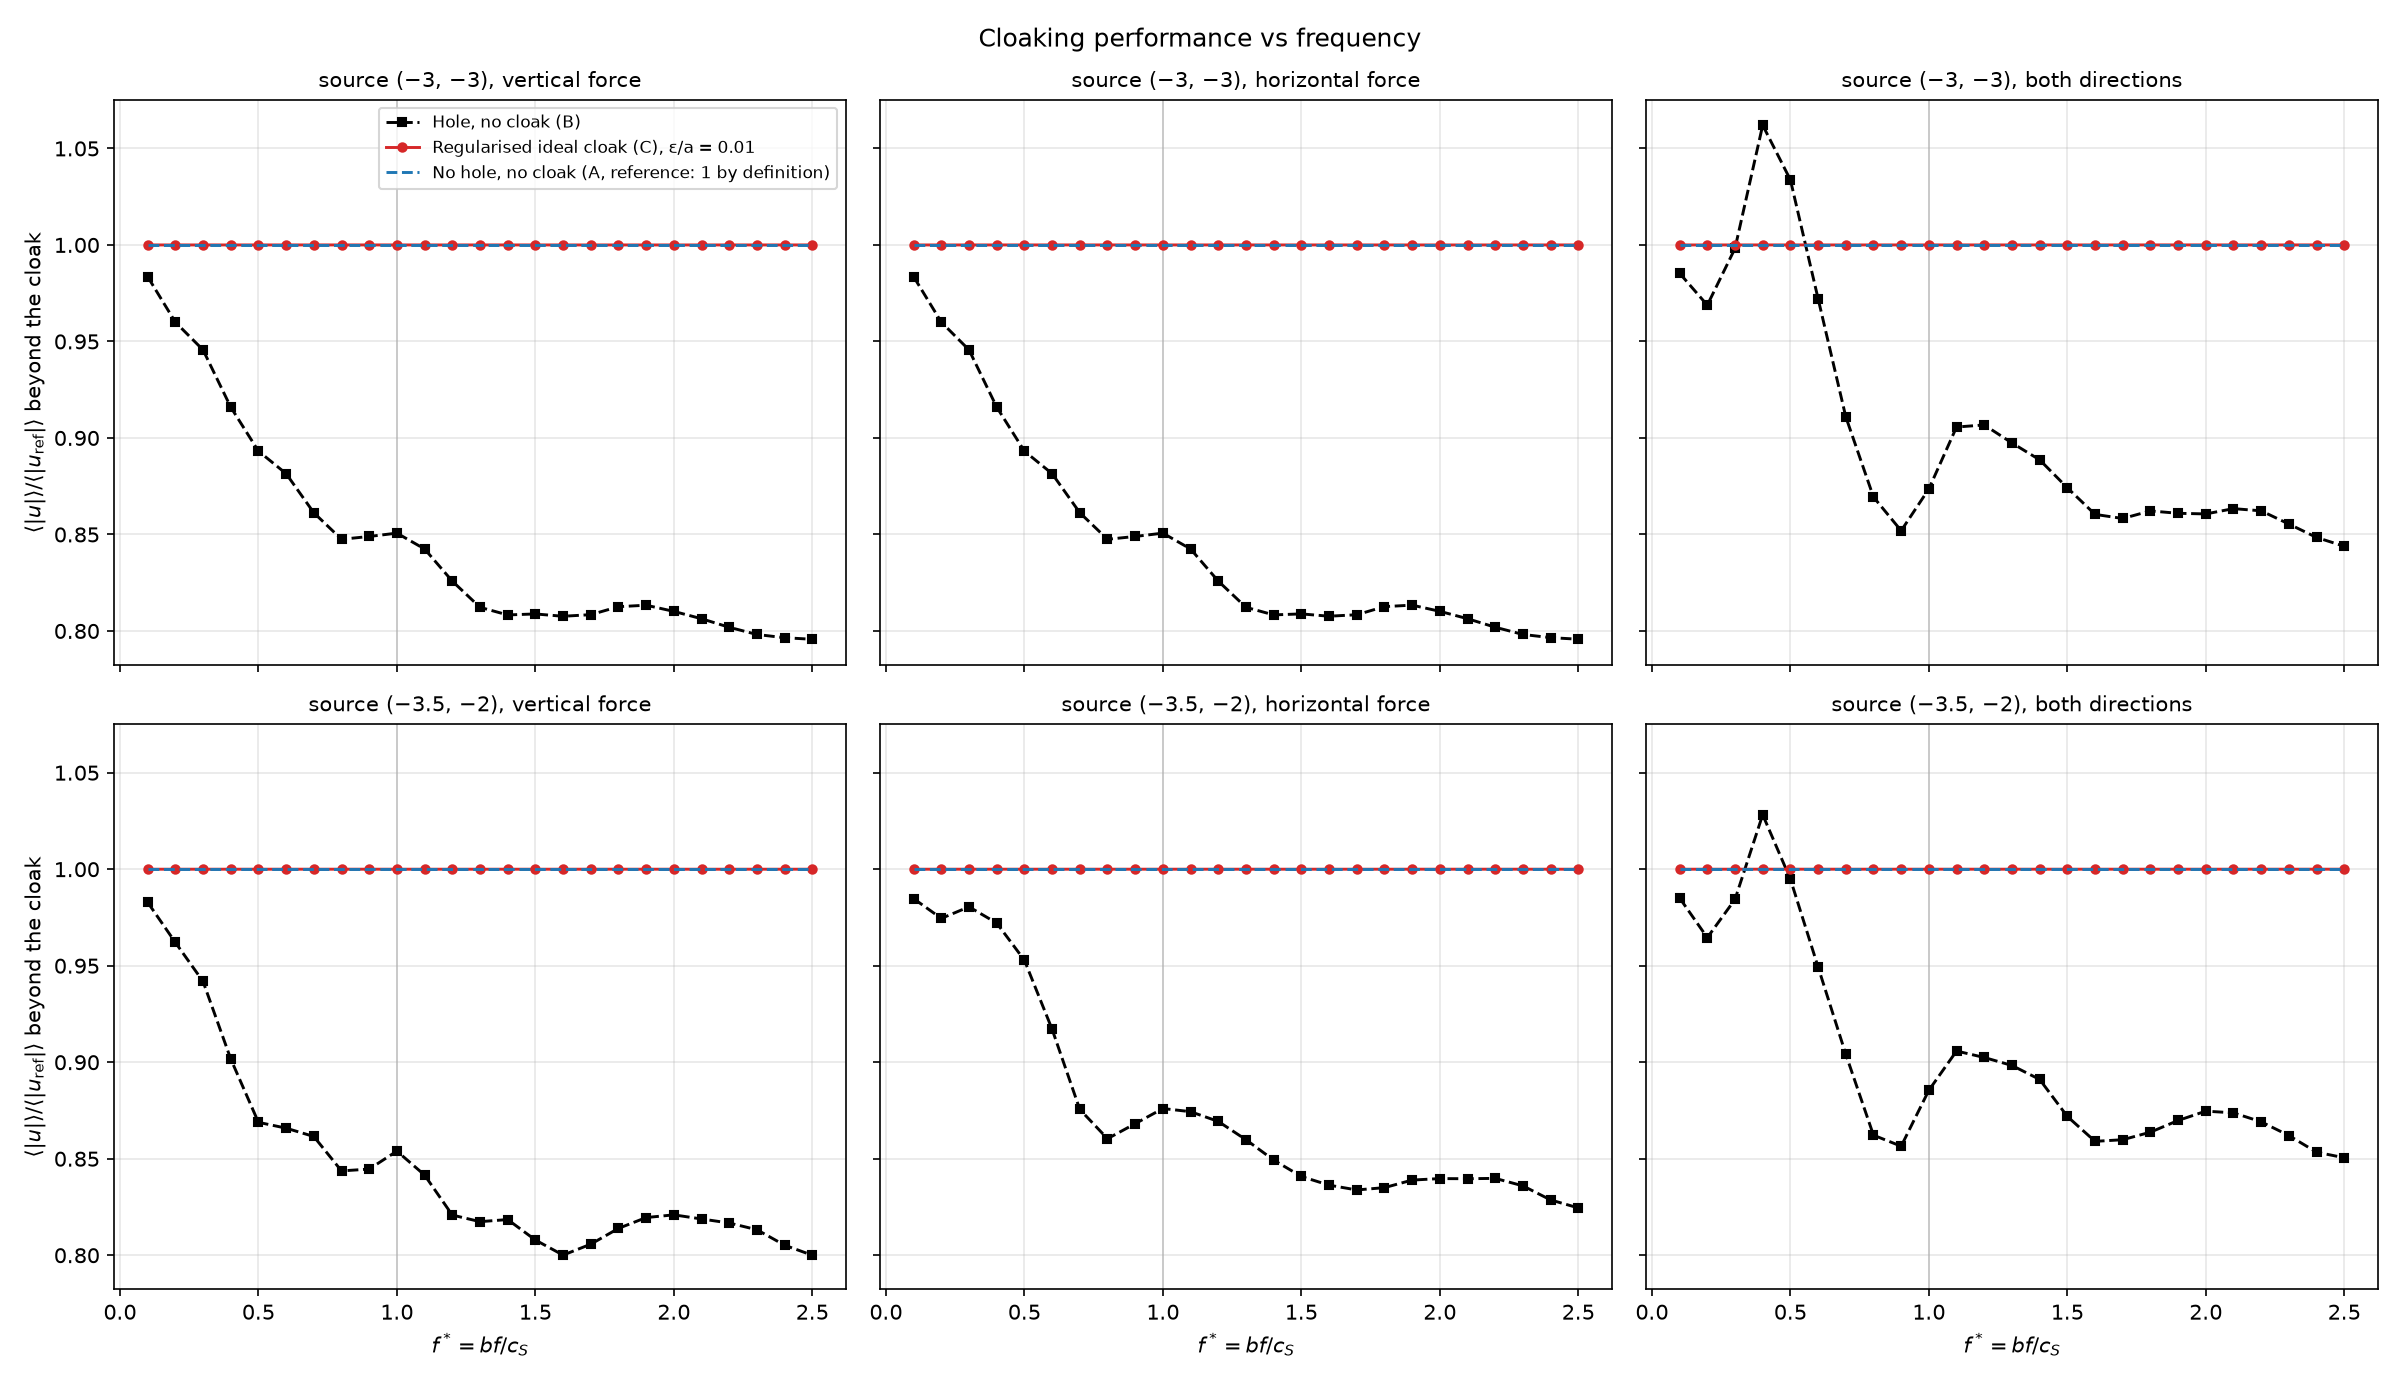
\includegraphics[width=\textwidth]{frequency_sweep_ratio.png}
\caption{Ratio $\eta$ of~\eqref{eq:eta} against frequency, beyond the cloak. Case A is 1 by definition; C overlaps it.}
\label{fig:sweepratio}
\end{figure}

\begin{figure}[!htb]
\centering
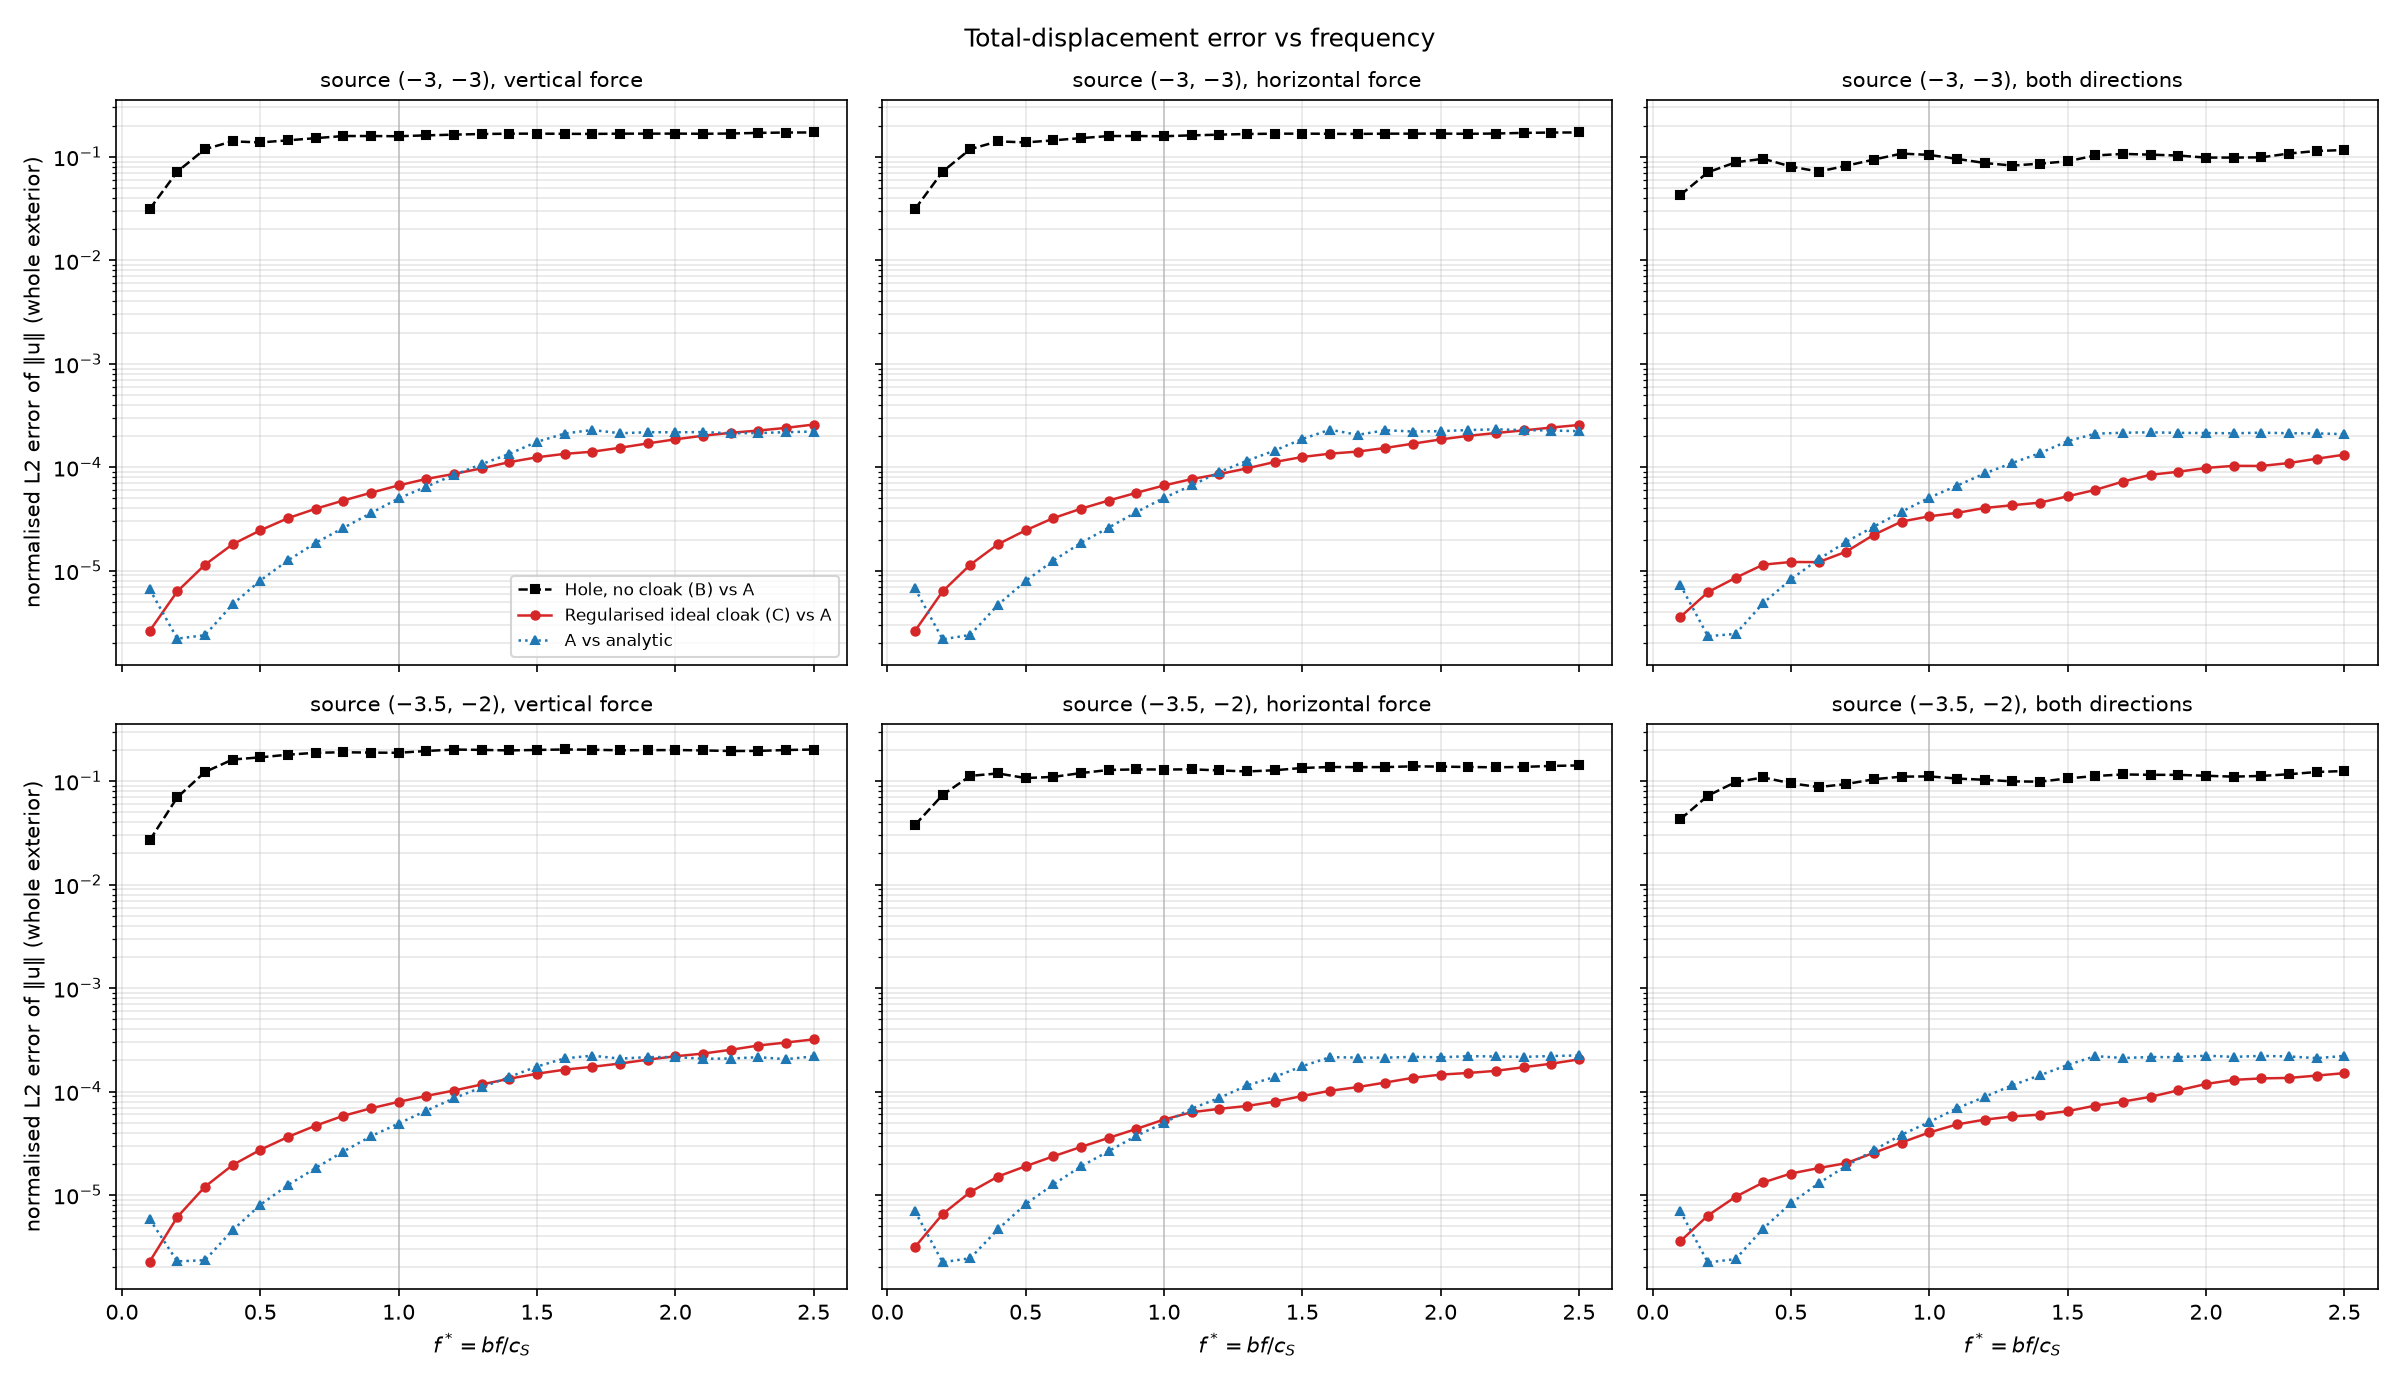
\includegraphics[width=\textwidth]{frequency_sweep_error.png}
\caption{Magnitude error over the whole exterior against frequency.}
\label{fig:sweeperror}
\end{figure}

\begin{figure}[!htb]
\centering
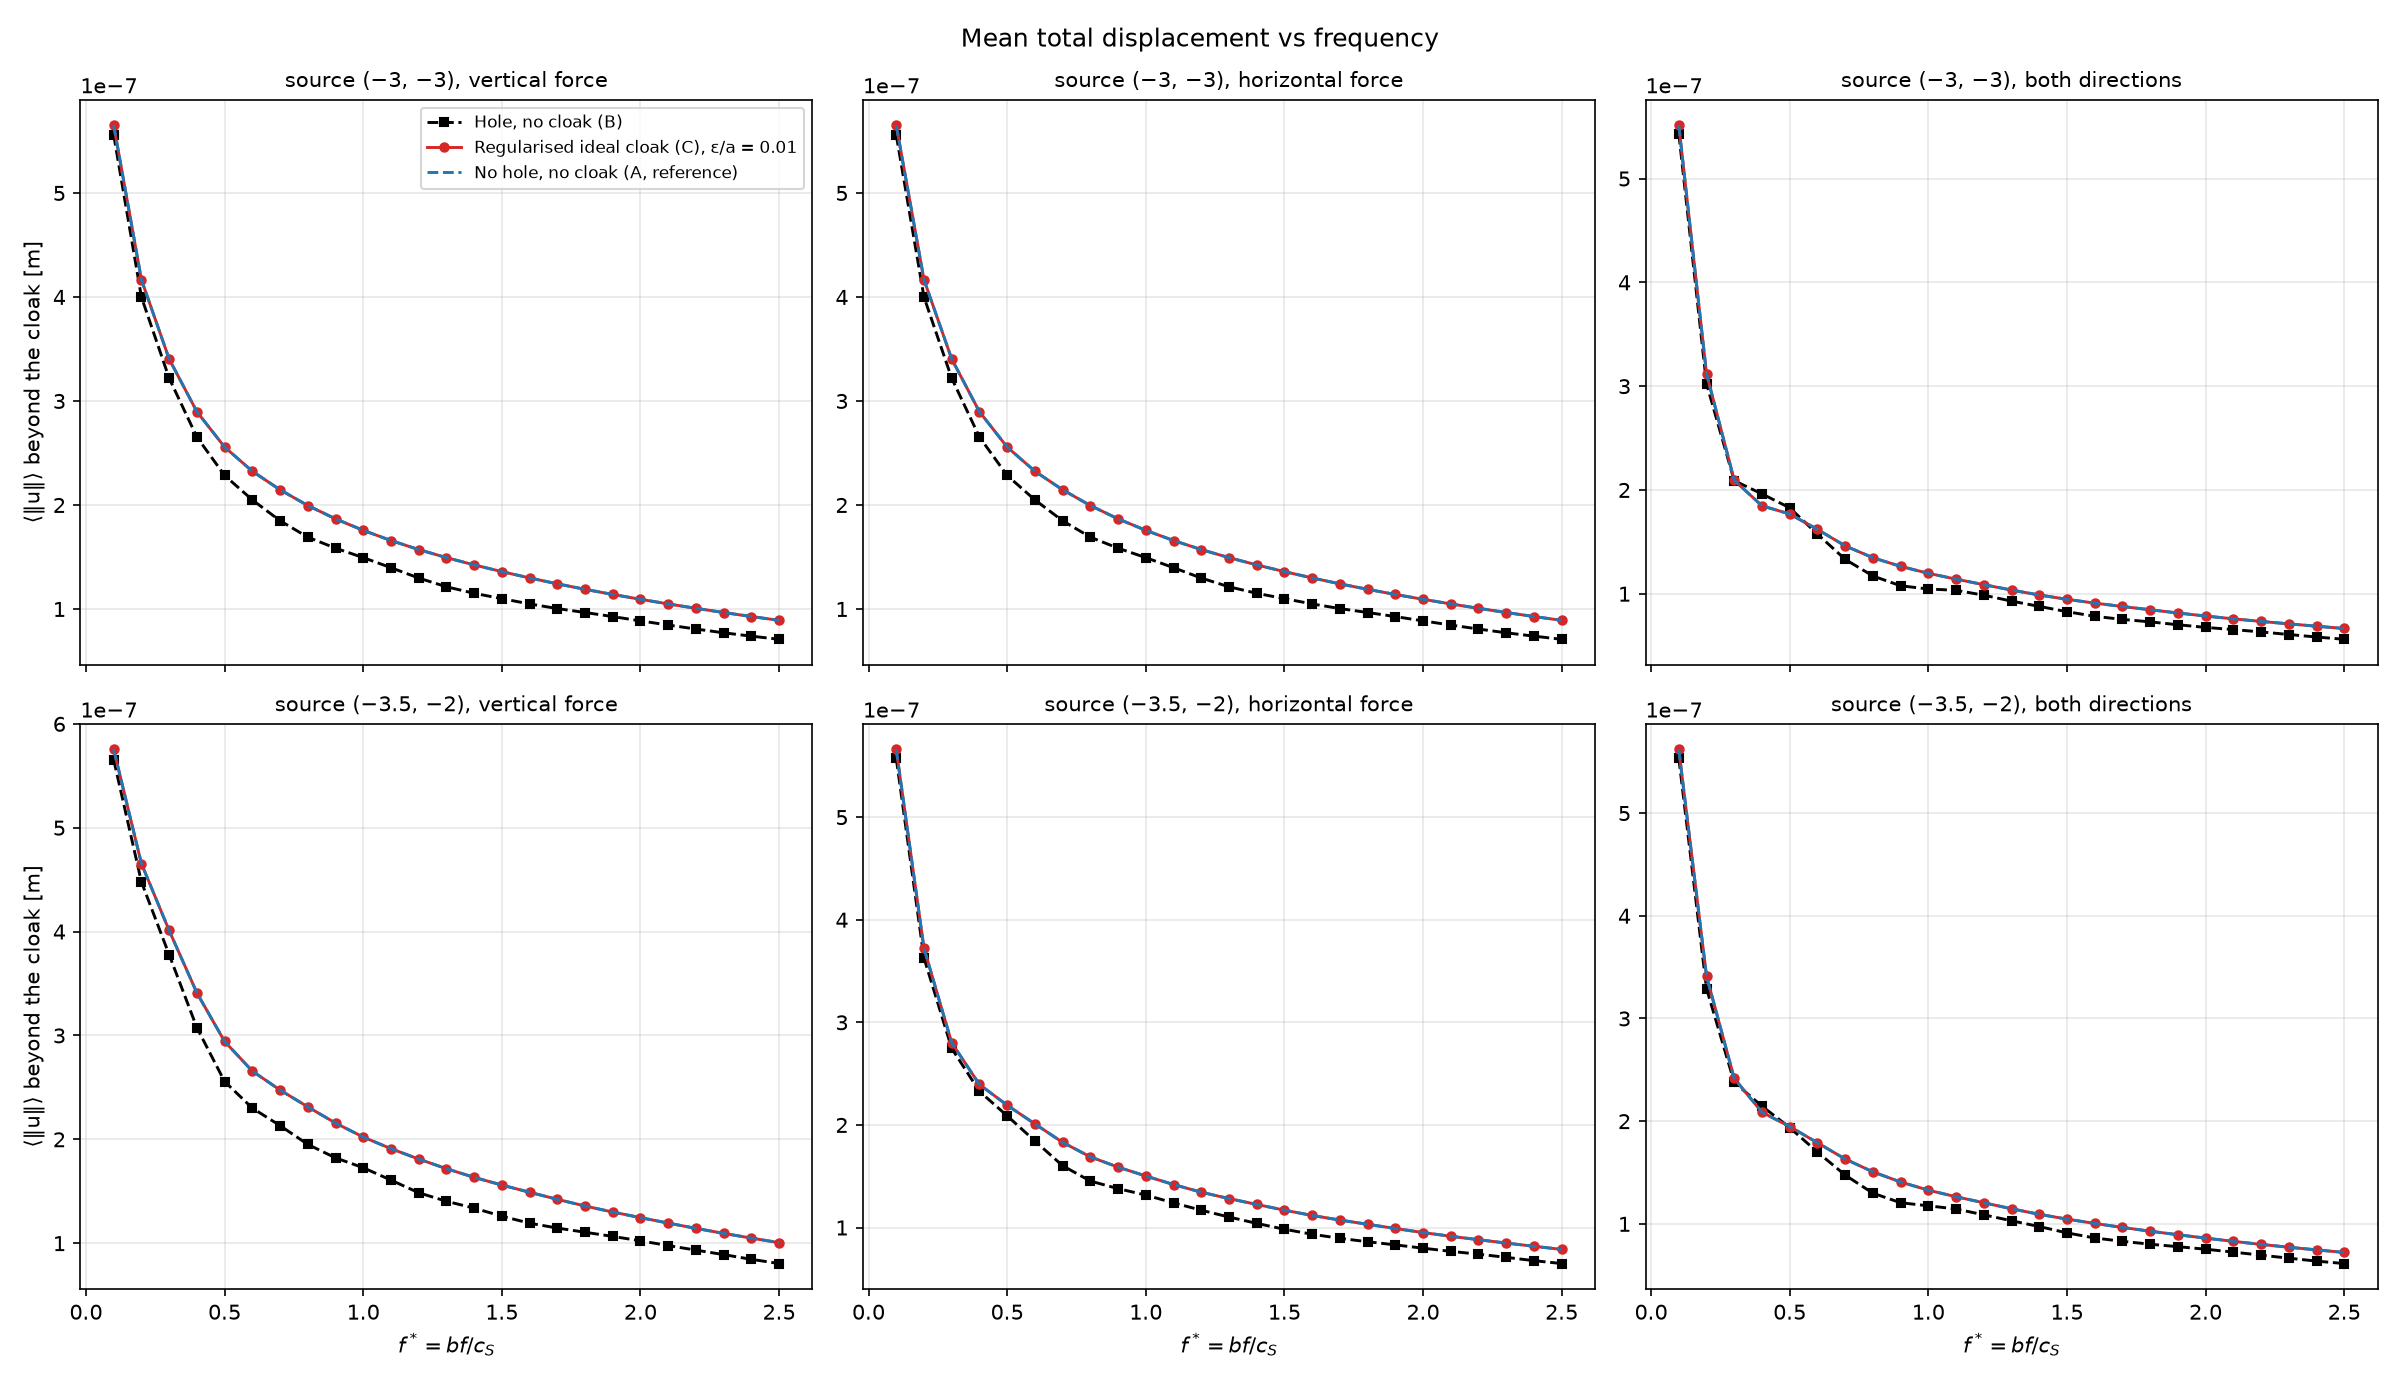
\includegraphics[width=\textwidth]{frequency_sweep_mean_displacement.png}
\caption{Absolute mean total displacement beyond the cloak against frequency. Curves A and C overlap.}
\label{fig:sweepmean}
\end{figure}

\begin{figure}[!htb]
\centering
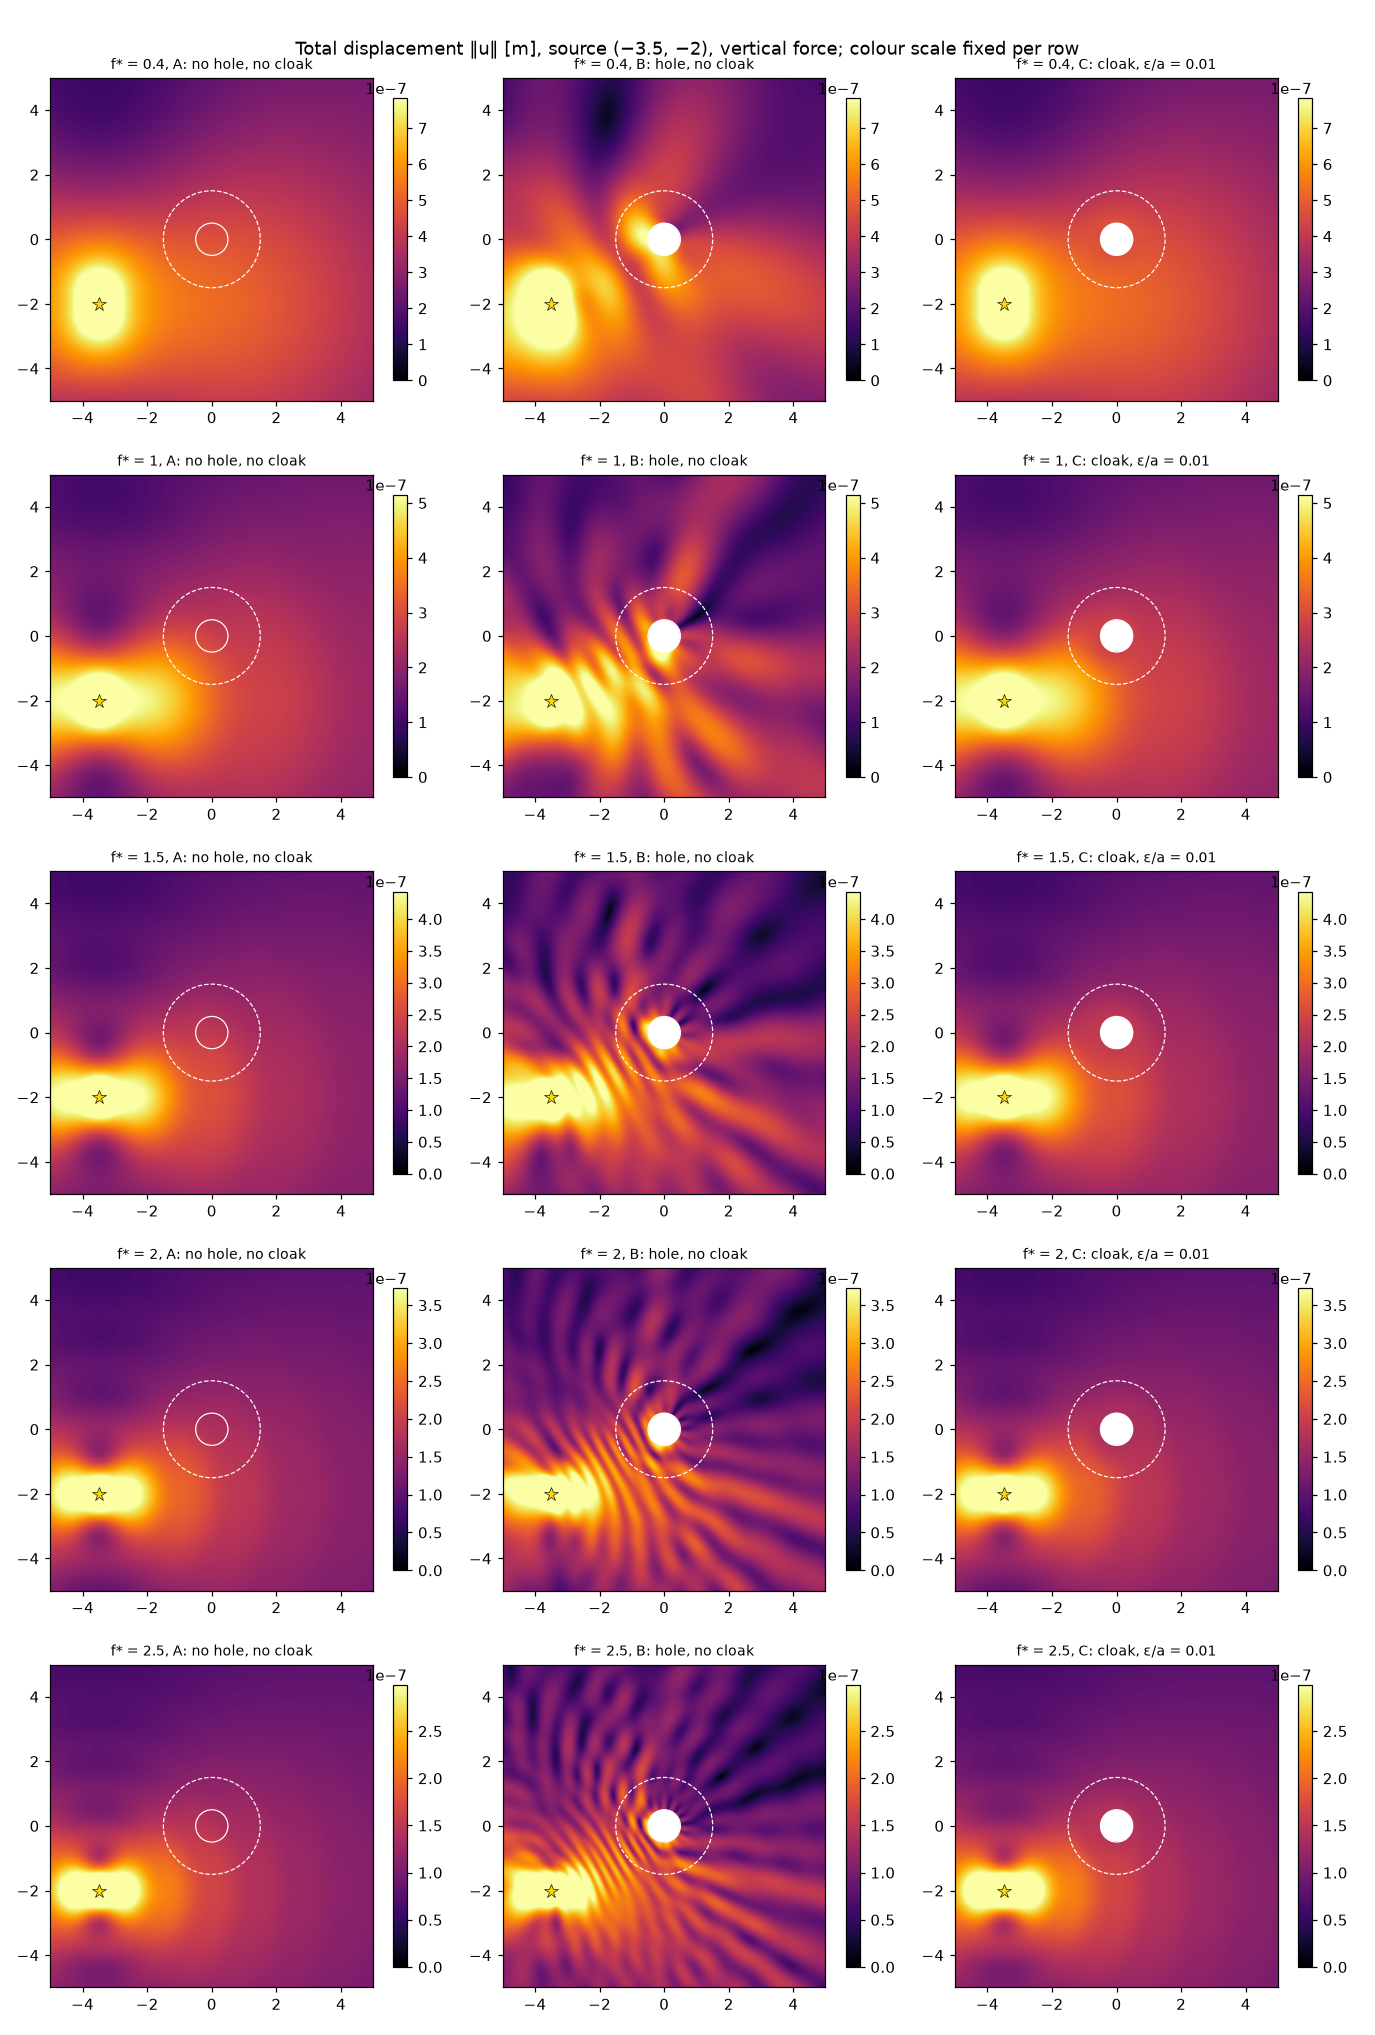
\includegraphics[width=0.74\textwidth]{overview_off_diagonal_vertical.png}
\caption{Total displacement at $f^*=0.4,1,1.5,2,2.5$ for the source $(-3.5,-2)$\,m and vertical force. Columns: A, B, C. Colour scale fixed per row.}
\label{fig:overview}
\end{figure}

\FloatBarrier
\subsection{Why the ratio can exceed one}\label{sec:ratio}

The bare-hole ratio is not bounded by 1. For $\hat{\mbf{d}}=(1,1)/\sqrt{2}$ at source $(-3,-3)$\,m, it reaches $\eta_B=1.062$ at $f^*=0.4$, with a smaller peak of $1.028$ at $(-3.5,-2)$\,m (Fig.~\ref{fig:sweepratio}). This is not a numerical artefact, since A agrees with the closed form to about $5\times10^{-6}$ there, and C stays at 1. To explain it, write $\mathbf{u}_{\mathrm{sc}}=\mbf{u}_B-\mbf{u}_A$ and use
\be\label{eq:energy}
  \|\mbf{u}_B\|^2-\|\mbf{u}_A\|^2=\|\mbf{u}_{\mathrm{sc}}\|^2+2\,\mathrm{Re}\bigl(\mbf{u}_A^{*}\cdot\mbf{u}_{\mathrm{sc}}\bigr).
\ee
Table~\ref{tab:diagnostic} evaluates the two terms beyond the cloak. Scattered fields of comparable size add a similar energy for both forces. The difference at $f^*=0.4$ lies in the interference: $-0.276$ for the vertical force, which forms a shadow, but only $+0.001$ for the combined force, whose scattered energy simply adds. In that case the force points along the source--cloak axis, near which the S radiation of a point force is weak, so the reference field is dominated by P waves (64\% of the energy) and is about one third smaller. A plausible reason for the absence of the shadow is the long P wavelength, $\lambda_P=6.5$\,m, relative to the 1\,m hole, but we did not isolate this cause. At $f^*=1$, interference becomes strong in both cases and $\eta_B<1$.

There is no conflict with energy conservation, since $\eta$ is a mean amplitude over one region and not a flux. More generally, $\eta$ is a weak metric for embedded cavities: it remains within about 20\% of 1 here, while the error $e_B$ reaches 0.20 and the maps of Fig.~\ref{fig:overview} show strong scattering. We therefore regard $e$ as the primary evidence.

\begin{table}[!htb]
\centering\footnotesize
\caption{Decomposition~\eqref{eq:energy} beyond the cloak for the bare hole at source $(-3,-3)$\,m, where the off-axis distance is $d_\perp$.}
\label{tab:diagnostic}
\resizebox{\textwidth}{!}{\begin{tabular}{lcccc}
\toprule
 & $f^*=0.4$, V & $f^*=0.4$, both & $f^*=1$, V & $f^*=1$, both \\
\midrule
$\eta_B$ beyond the cloak & 0.916 & 1.062 & 0.851 & 0.874 \\
\quad near the axis, $|d_\perp|<2$\,m & 0.795 & 1.024 & 0.713 & 0.837 \\
\quad to the sides, $|d_\perp|\geq 2$\,m & 1.091 & 1.102 & 1.047 & 0.913 \\
P share of the energy of $\mathbf{u}_A$ & 0.16 & 0.64 & 0.17 & 0.67 \\
$\langle\|\mathbf{u}_A\|\rangle$ [$10^{-7}$\,m] & 2.90 & 1.85 & 1.76 & 1.20 \\
scattered energy $\langle\|\mathbf{u}_{\mathrm{sc}}\|^2\rangle/\langle\|\mathbf{u}_A\|^2\rangle$ & $+0.153$ & $+0.158$ & $+0.347$ & $+0.259$ \\
interference $2\langle\mathrm{Re}\,\mathbf{u}_A^*\!\cdot\mathbf{u}_{\mathrm{sc}}\rangle/\langle\|\mathbf{u}_A\|^2\rangle$ & $-0.276$ & $+0.001$ & $-0.574$ & $-0.441$ \\
\bottomrule
\end{tabular}
}
\end{table}

%% =============================================================
\FloatBarrier
\section{Discussion}\label{sec:discussion}
%% =============================================================

Theorem~\ref{thm:equivalence} turns the assessment of a regularised cloak into the comparison of two ordinary problems. Without case D, a small value of C vs.\ A alone would not tell whether the residual comes from $\varepsilon$ or from the discretisation. Here the decomposition shows that it comes from $\varepsilon$ at the base resolution, and that the numerical error is smaller. The comparison of layers also shows why a validation against an analytic reference is needed in addition: the original damping layer had a 3.5\% complex error against~\eqref{eq:green}, invisible in C vs.\ A.

Our results have the following limits. Only two source positions were considered, with frequency up to $b/\lambda_S=2.5$ and one geometry, $b=3a$. Refinement near the cavity and quadrature order were not studied separately, and the behaviour of C vs.\ D on finer meshes remains open. Case B has no independent reference such as a series solution for the cavity. The PML was tested through its effect on case A, and the elastodynamic stability of the layer was not analysed beyond the frequency-domain results. The medium~\eqref{eq:pushforward} has strong contrast at small $\varepsilon$ and broken minor symmetry, up to about 0.45 in the relative measure of Fig.~\ref{fig:material}, and we have not addressed how it would be realised.

The natural next step is to approximate this continuous reference by a limited number of piecewise-constant material pixels, first to measure the pixelisation error alone, then to optimise admissible Cauchy materials against the metrics used here. Those stages are future work and no results for them are reported here.

%% =============================================================
\section{Conclusion}\label{sec:conclusion}
%% =============================================================

We have formulated and validated a regularised continuous cloak for a circular cavity embedded in an elastic medium and excited by bulk waves. An exact equivalence with a hole of radius $\varepsilon$ yields a direct way of separating regularisation and numerical errors, and implies traction continuity at the outer interface for any increasing $C^1$ radial map. With a stretched-coordinate PML and quadratic elements, the model agrees with a closed-form reference and satisfies superposition and mirror identities. For $b=\lambda_S$ and $\varepsilon/a=0.01$, the cloak reduces the normalised exterior error in total displacement from $0.158$ to $6.7\times10^{-5}$. The error scales as $\varepsilon^2$, and remains below $3.2\times10^{-4}$ for all force directions, source positions and frequencies tested. These results provide a verified baseline for realisable approximations of the cloak.

\section*{Data availability}
The code, configurations and result tables are in the \texttt{circular\_cloak} branch of the project repository. The drivers are the following files in its \texttt{scripts} directory:
\begin{itemize}
\item \texttt{circular\_step1.py}
\item \texttt{circular\_frequency\_sweep.py}
\item \texttt{circular\_ratio\_diagnostic.py}
\end{itemize}

%% TODO: CRediT authorship contribution statement, declaration of competing interest, acknowledgements and funding.

\bibliographystyle{elsarticle-num-names}
\bibliography{refs}

\end{document}
